\documentclass[a4paper,12pt,liststotoc,DIV12]{scrartcl}
%\usepackage{geometry}
%\usepackage{ngerman}
\usepackage{longtable}
\usepackage[T1]{fontenc}
\usepackage{ae}
\usepackage[utf8]{inputenc}
\usepackage{fancyhdr}
\usepackage{graphicx}
\usepackage{xspace}
\usepackage[cmyk]{xcolor}
\usepackage{amsmath}
\usepackage[
  %plainpages=false,
  %pdfpagelabels,
  %colorlinks=true,
  pdfborder={0 0 0},
  %urlcolor=blue,
  %linkcolor=blue,
  bookmarksopen=true,
  %pdfstartpage=3,
  unicode,
]{hyperref}
\hypersetup{
  pdftitle={OST-WeST - Detailed Design},
  pdfsubject={OST-WeST - Detailed Design},
  pdfauthor={Stefan Franke, Robert Hanussek, Benjamin Keil, Steffen Kieß, Johannes Langauf, Christoph Marian Müller, Igor Podolskiy, Tilmann Scheller, Michael Starzmann, Markus Wittlinger},
  pdfkeywords={OST-WeST, Detailed Design},
}
% hypcap is needed for correct links to figures, see specification Bug 2
\usepackage[all]{hypcap}
\usepackage{svnkw}
\usepackage[USenglish]{isodate}
\usepackage{titlesec}
% provides \ul,  allows line breaking for underlined text (static methods...)
\usepackage{soul}
\makeatletter

% some TeX voodoo to extract the date from SVN ID
% which can be processed by isodate 
\def\svn@dateonly#1 #2Z{#1}
\def\svndateonly#1{%
\ifx#1\empty1970-01-01\else
\expandafter\svn@dateonly#1\fi}

% Two-level figure & table numbering
\@addtoreset{table}{section}
\@addtoreset{figure}{section}
\renewcommand{\thefigure}{\thesection.\arabic{figure}}
\renewcommand{\thetable}{\thesection.\arabic{table}}
\makeatother

% custom font sizes for headings, non run-in titles for [sub]paragraphs
\titleformat{\section}{\bfseries\fontsize{24}{30}\selectfont\sffamily}{\thesection}{1em}{}
\titleformat{\subsection}{\bfseries\fontsize{18}{24}\selectfont\sffamily}{\thesubsection}{1em}{}
\titleformat{\subsubsection}{\bfseries\fontsize{16}{22}\selectfont\sffamily}{\thesubsubsection}{1em}{}
\titleformat{\paragraph}{\bfseries\fontsize{14}{20}\selectfont\sffamily}{\theparagraph}{1em}{}
\titleformat{\subparagraph}{\bfseries\normalsize\sffamily}{\thesubparagraph}{1em}{}
\titlespacing{\paragraph}{0pt}{\parskip}{-0.5\parskip}{}
\titlespacing{\subparagraph}{0pt}{\parskip}{-0.5\parskip}{}

\svnid{$Id: DetailedDesign.tex 1 2007-12-12 17:37:26Z t-scheller $}

\parindent0mm
\parskip2mm
%\geometry{textwidth=160mm, textheight=230mm, inner=30mm}

\xdefinecolor{TodoColor}{rgb}{1.0, 0.0, 0.0}

% depth of the headlines that are numbered
\setcounter{secnumdepth}{5}
\setcounter{tocdepth}{5}

\newcommand{\OSTWeST}{\textit{OSTWeST}\xspace}
\newcommand{\gbt}{\textit{gbt$^2$}\xspace}
\newcommand{\eclui}{\textsf}
\newcommand{\code}{\texttt}
\newcommand{\todo}[1]{\bgroup\color{TodoColor}\textsc{\textbf{TODO:} #1}\egroup}
\newcommand{\BIG}{\fontsize{48}{48}\selectfont}
\newcommand{\linkwithfootnote}[2]{\href{#1}{#2}\footnote{\url{#1}}}
\newcommand{\email}[1]{\href{mailto:#1}{#1}}

\xdefinecolor{ClassColor}         {rgb}{0.0, 1.0, 0.0}
\xdefinecolor{ClassAbstractColor} {rgb}{0.0, 1.0, 0.0}
\xdefinecolor{ObjectColor}        {rgb}{0.31, 0.58, 0.84}
\xdefinecolor{InterfaceColor}     {rgb}{1.0, 0.0, 1.0} % that's magenta NOT pink, OK? ;-)
\xdefinecolor{ImplementerColor}   {rgb}{0.4, 0.2, 0.6}
\xdefinecolor{FieldColor}         {rgb}{0.9, 0.5, 0.0}

\newcommand{\pkg}[1]{\texttt{#1}}
\newcommand{\cls}[1]{\texorpdfstring{{\color{ClassColor}\texttt{#1}}}{#1}}
\newcommand{\clsab}[1]{\texorpdfstring{{\color{ClassAbstractColor}\textit{\texttt{#1}}}}{#1}}
\newcommand{\obj}[1]{\texorpdfstring{{\color{ObjectColor}\texttt{#1}}}{#1}}
\newcommand{\itf}[1]{\texorpdfstring{{\color{InterfaceColor}\texttt{#1}}}{#1}}
\newcommand{\imp}[1]{\texorpdfstring{{\color{ImplementerColor}\texttt{#1}}}{#1}}
\newcommand{\mtd}[1]{\texttt{#1}}
\newcommand{\mtdst}[1]{\texorpdfstring{\ul{\texttt{#1}}}{#1}}
\newcommand{\mtdab}[1]{\texorpdfstring{\textit{\texttt{{#1}}}}{#1}}
\newcommand{\fld}[1]{{\color{FieldColor}\texttt{#1}}}
\newcommand{\namespace}[1]{\begin{description}\item[Namespace:]#1\end{description}}
\newcommand{\rootpkg}{org.gbt2}


\newcommand{\codepageflag}{iscodecontainer}

% needed for the Function Point tables
\newcommand{\x}{\textbullet}

%\includeonly{Introduction}
%\includeonly{UserInterface}
%\includeonly{FunctionalRequirements}
%\includeonly{NonFunctionalRequirements}
%\includeonly{Conclusion}
\begin{document}

% --- title page --- %
\pagestyle{empty}
\begin{titlepage}
 \vspace*{38mm}
 \begin{center}
 \fontsize{24}{24}\selectfont
 Detailed Design\\
 \vspace*{12mm}
 \fontsize{48}{48}\selectfont
 
 % gross hack to generate the a big fancy gbt-squared appearance
 \textit{gbt}$\fontsize{32}{32}\fontfamily{ptm}\selectfont ^\textit{2}$
 %
 \\
 \fontfamily{\familydefault}\fontsize{32}{38}\selectfont
 Glass Box Testing Tool\\
 \vspace*{12mm}
 \fontsize{16}{20}\selectfont
 Student Project A ``OST-WeST''\\
 University of Stuttgart

 \vspace{2cm}
 {\small 
   Version: 1.2 \\
   {Last changed on \printdate{\svndateonly{\svndate}} (SVN Revision \svnrev)}}
   \end{center}
   \vspace{3cm}
   \hspace{40mm}
   \normalsize
\end{titlepage}

% --- Header and version history --- %

\cleardoublepage
\fancyhf{}
\fancyhead[RE,LO]{\textit{\gbt - Design}}
\fancyhead[RO,LE]{\thepage}
\pagestyle{fancyplain}

% -- Version History -- %
\svnid{$Id: VersionHistory.tex 23 2008-05-28 11:39:25Z ahija $}

\section*{Version History}

{\small
\begin{longtable}{|l|l|p{35mm}|p{71mm}|} \hline
   {\normalsize \textbf{Date}} &
   {\normalsize \textbf{Version}} &
   {\normalsize \textbf{Author}} & 
   {\normalsize \textbf{Modifications}} \\\hline \hline \endhead
    11.01.2007 &  0.1 &  Stefan Franke & 
      - Chapter files and master document file \\\hline
    16.01.2007 &  0.2 &  Stefan Franke & 
      - ui: Eclipse Plug-in and images within \\\hline
    17.01.2007 &  0.3 & Michael Starzmann \newline Christoph Müller & 
      - Headwords following the corresponding chapter in the analysis-notes \newline
      - nr: Keywords taken over by the analysis notes \newline
      - fr: The foreword for the functional requirements \\\hline
    18.01.2007 &  0.4 &  Stefan Franke & 
      - ui: Rewrite source code highlighting \newline
      - Reorder chapters \newline
      - Rename some sections \newline
      - ui: Added source code highlighting for COBOL \\\hline
    19.01.2007 &  0.5 &  Christoph Müller & 
      - Document structure changed \newline
      - fr: Use case pictures imported \newline
      - fr: Foreword, fr: actors, fr: general arrangements \\\hline
    20.01.2007 & 0.6 & Johannes Langauf \newline Christoph Müller & 
      - nf: Expand some keywords to complete sentences \newline
      - nf: Find new NFRs \newline
      - fr: Configuration \newline
      - fr: Use case description \newline
      - fr: Language support \\\hline
    21.01.2007 & 0.7 & Christoph Müller \newline Stefan Franke & 
      - fr: Use case description \newline
      - ui: Session view, Coverage view and Launching \\\hline
    23.01.2007 & 0.8 & Christoph Müller \newline Stefan Franke \newline Michael Starzmann& 
      - Correction after specification meeting \newline
      - fr: Use case description of measure coverage \newline
      - fr: General functional requirements \newline
      - fr: Reports \newline
      - ui: Configuration dialogs \\\hline
    24.01.2007 & 0.9 & Michael Starzmann \newline Christoph Müller & 
      - in: Introduction \newline
      - fr: Use case description \newline
      - fr: Coverage Criteria \\\hline
    25.01.2007 & 0.10 & Michael Starzmann \newline Stefan Franke & 
      - ui: Package and file selection to ... states \newline
      - fr: Coverage measurement improved \newline
      - in: Introduction \\\hline
    26.01.2007 & 0.11 & Christoph Müller \newline Stefan Franke & 
      - Correction after specification meeting \newline
      - fr: New use case instrument instrumentable items \newline
      - ui: Configuration sections \newline
      - ui: Source code highlighting \\\hline
    27.01.2007 & 0.12 & Christoph Müller \newline Stefan Franke \newline Michael Starzmann & 
      - fr: Use case description of administrate sessions \newline
      - ui: Instrumentation subsection \newline
      - ui: Solved todos \newline
      - ui: first draft for the Batch interface \newline
      - fr: Release, folders, files \\\hline
    28.01.2007 & 0.13 & Christoph Müller \newline Stefan Franke \newline Johannes Langauf & 
      - fr: Batch interface \newline
      - ui,fr: Correction after internal review \newline
      - nr: improve and fill out most non-functional requirements \\\hline
    29.01.2007 & 0.14 & Christoph Müller & 
      - fr: Solve todos, use case diagrams, folder structure \newline
      - Correction after QA meeting \newline
      - small spell check \\\hline
    30.01.2007 & 0.15 & Christoph Müller \newline Stefan Franke \newline Johannes Langauf & 
      - fr: New use cases: analyse coverage log, export session \newline
      - ui: New Context menu \newline
      - ui: Import, Export, Report \newline
      - ui: Small adaption at figures \newline
      - nf: Correction after specification review \newline
      - nf: Extensibility, performance requirements, program examples \\\hline
    31.01.2007 & 0.16 & Christoph Müller \newline & 
      - Correction after Igor's big bang \\\hline
    31.01.2007 & 1.0 & Igor Podolskiy & Declaring version 1.0, ready for review \\\hline
    08.02.2007 & 1.1-dev-1 & Stefan Franke \newline Michael Starzmann & 
      - Correction after specification review \\\hline
    09.02.2007 & 1.1-dev-2 & Christoph Müller & 
      - Correction after specification review \\\hline
    10.02.2007 & 1.1-dev-3 & Christoph Müller & 
      - Correction after specification review: Bugs 47, 90, 52, 57, 56, 58, 60, 62, 63, 64, 65, 39, 40, 41, 42, 44, 46, 50, 51, 52, 54, 34 \\\hline
    11.02.2007 & 1.1-dev-4 & Johannes Langauf \newline Christoph Müller \newline Stefan Franke & 
      - Correction after specification review: Bugs 48, 35, 32, 91, 16 \\\hline
    12.02.2007 & 1.1-dev-5 & Johannes Langauf \newline Christoph Müller  &
      - Correction after specification review: Bug 22 \newline
      - new batch commands \\\hline
    13.02.2007 & 1.1-dev-6 & Stefan Franke \newline Christoph Müller &
      - moved the glossary to specification document \newline
      - added links to glossary entries \newline
      - Bug 7: Work flow \newline
      - Bugs 6, 21, 28, 88, 89, 91\\\hline
    14.02.2007 & 1.1-dev-7 & Stefan Franke \newline Christoph Müller \newline Michael Starzmann &
      - Bug 45 \\\hline
    16.02.2007 & 1.1-dev-8 & Stefan Franke \newline Christoph Müller &
      - Bug 45 \\\hline
    11.05.2007 & 1.1-dev-9 & Stefan Franke \newline Christoph Müller &
      - Bugs 98, 99, 100 \\\hline
    15.06.2007 & 1.1-dev-10 & Christoph Müller & 
      - fr: \ref{fr:JUnit integration} JUnit integration \\\hline
    17.06.2007 & 1.1-dev-11 & Stefan Franke & 
      - ui: \ref{ui:Boolean Analyzer} Boolean Analyzer \\\hline
    18.06.2007 & 1.1-dev-12 & Christoph Müller & 
      - fr: \ref{fr: Coverage measurement} coverage log file name \newline
      - fr: \ref{fr:Batch:Instrument} instrument supports a charset  \newline
      - fr: \ref{fr:Batch:Analyze} analyze supports a charset \newline
      - fr: \ref{fr:Batch:Instrumenter-info} Instrumenter-info \\\hline
    19.06.2007 & 1.1-dev-13 & Christoph Müller & 
      - fr: \ref{fr:Batch:Instrument} instrument has \verb$--$copy-uninstrumented \\\hline
    29.06.2007 & 1.1-dev-14 & Christoph Müller & 
      - fr: \ref{fr:Batch:Instrument} instrument has include, exclude \\\hline
    19.09.2007 & 1.1-dev-15 & Johannes Langauf & 
      - ui: \ref{ui:Hot-Path} Hot-Path: make outstanding decisions, update for configureable colors \newline
      - fr: remove PDF-Report support \\\hline
     31.10.2007 & 1.1-dev-16  & Tilmann Scheller  & general update of specification
       \\\hline
    28.05.2008 & 1.1-dev-17 & Christoph Müller & 
      - fr: \code{return} and \code{break} are basic statements too \\\hline
%     &   &   & 
%       \\\hline
\end{longtable}
}

%%% Local Variables: 
%%% mode: latex
%%% TeX-PDF-mode: t
%%% TeX-master: "Specification.ltx"
%%% End: 


% \cleardoublepage

% --- Table of contents --- %

\parskip1mm
\tableofcontents
\parskip2mm

\pagestyle{fancyplain}
\renewcommand{\baselinestretch}{1.25}\normalsize
\svnid{$Id: Introduction.tex 1 2007-12-12 17:37:26Z t-scheller $}
\section{Introduction} \label{Introduction}

\subsection{Project overview} \label{in:Overview}
\gbt is a glass box testing tool to measure the coverage of a running program.
It will be as independent as possible of the programming language of the covered program.

%TODO: Bla Bla bla...
\subsection{About this document} \label{in:AboutThisDocument}

This document contains the necessary information to create a detailed design
obeying the requirements documented in the specification. It describes the
behaviour of the software and the artifacts which are created by it. The
architecture is also defined by this document, as well as the data structures
used to store the data pertaining to the operation of the software. Details
like the structure of classes and the design of methods have to be determined
in the detailed design document.


\subsection{Addressed audience} \label{in:Addressed audience}
This document is addressed to
\begin{itemize}
  \item the customer who ordered the software
  \item the project manager controlling the work
  \item the quality assurance division creating test cases for the software
  \item the developers implementing the design
  \item future developers maintaining and extending the software
  \item interested users of the software
  \item students of upcoming student projects
\end{itemize}

\subsection{Authors}
In the following table authors of this document are named.
{\small
\begin{longtable}{|p{35mm}|p{65mm}|l|} \hline
   {\normalsize \textbf{Author}} &
   {\normalsize \textbf{E-mail}} \\\hline \hline \endhead
   Robert Hanussek & \email{hanussrt@studi.informatik.uni-stuttgart.de} \\\hline
   Steffen Kieß & \email{kiesssn@studi.informatik.uni-stuttgart.de} \\\hline
   Tilmann Scheller & \email{schellrt@studi.informatik.uni-stuttgart.de} \\\hline
   Markus Wittlinger & \email{wittlims@studi.informatik.uni-stuttgart.de} \\\hline
\end{longtable}
}




\subsection{Notation}

\subsubsection{Identifiers}

\cls{FooBar} denotes a class named \code{FooBar}.

\clsab{FooBar} denotes an abstract class named \code{FooBar}.

\obj{FooBar} denotes an instantiated object of class \cls{FooBar}.

\itf{FooBar} denotes an interface class named \code{FooBar}.

\imp{FooBar} denotes an object of a class which implementes the interface named \code{FooBar}.

\mtd{fooBar(...)} denotes a method named \code{fooBar} which has parameters (which are not listed). Methods don't have a special color because they can be easily identified by the trailing brackets.

\mtd{fooBar()} denotes a method named \code{fooBar} which doesn't have any parameters.

\mtdst{fooBar(...)} denotes a static method (which has parameters).

\fld{fooBar} denotes a field named \code{fooBar}.

\pkg{foo.bar} denotes a package called \code{bar} which resides in a package called \code{foo}. Packages don't have a special color because they can be identified easily since they are the only items which contain a dot and are lower case.

%% \subsubsection{Namespace}

%% Every section can define a namespace. All relative paths in such a section are relative to this namespace except paths which point to standard Java classes which are listed below. If for example the namespace \pkg{\rootpkg.report} is defined then \pkg{html.}\cls{Report} points to class \cls{Report} which resides in the package \pkg{\rootpkg.report.html}. It is also possible to define namespaces which refer to classes, e.g. \pkg{\rootpkg.report.}\cls{Report}. This allows it to directly reference the methods in \cls{Report} (see~\ref{Classes:Report:Report} for an example).

%% Namespaces are defined directly under the header of a section and are valid for the section the header belongs to. A Namespace definition looks like this:
%% \namespace{\pkg{\rootpkg.report}}

%% Following standard Java classes are used in this document without specifing their fully qualified package paths. These classes are also unaffected by namespace definitions:
%% % we will just write String instead of java.lang.String
%% \begin{itemize}
%% \item \pkg{java.lang.}\cls{String}
%% \item \pkg{java.io.}\cls{OutputStream}
%% \item \pkg{java.util.}\itf{List}
%% \end{itemize}

\svnid{$Id: Overview.tex 1 2007-12-12 17:37:26Z t-scheller $}
\section{UML-Model}
\linkwithfootnote{http://bouml.free.fr}{BOUML 2.21.5} was used to create the UML-Model. The BOUML files can be found in the subversion repository under \code{/svn/trunk/design/design/}. To avoid inconsistencies between this document and the model detailed in BOUML, no diagrams are included here, but all exist within the model. 
\section{Code examples}
Examples for instrumented Java- and COBOL-Code can be found in the subversion repository under \code{/svn/trunk/misc/instrumentation/code\_examples/}. The content of these files is not included here, because code examples are cumbersome and better readable in a normal text editor or IDE.
\section{Structural makeup of XML-Files}
\begin{verbatim}
<HierarchyLevel>
	<HierarchyLevelType englishName="" internalName=""/>
	<LocationList>
		<Location startOffset="" endOffset="">
			<SourceFile fileName="" content=""/>
		</Location>
	</LocationList>
	<StatementSequence>
		<BasicStatement>
			<CoverableItem id=""/>
			<RootTerm>
				<MapEntry>
					<BooleanAssignment>
						<BooleanResult value=""/>
						<BooleanResult value=""/>							<BooleanResult value=""/>
					</BooleanAssignment>
					<CoverableItem id=""/>
				</MapEntry>
				<BooleanTerm type="">
					<BooleanTerm type="">
					<BooleanOperator arity="" name=""/>
						<MapEntry>
							<BooleanAssignment>
								<BooleanResult value=""/>
								<BooleanResult value=""/>								<BooleanResult value=""/>
							</BooleanAssignment>
							<Boolean value="">
						</MapEntry>
					</BooleanTerm>
				</BooleanTerm>
			</RootTerm>
		</BasicStatement>
		<LoopingStatement optionalBodyExecution="" neverExecutedItemId="" onceExecutedItemId="" multipleExecutedItemId="">
			<LocationList>
				<Location startOffset="" endOffset="">
					<SourceFile fileName="" content=""/>
				</Location>
			</LocationList>
			<CoverableItem id=""/>
			<RootTerm/>
			<StatementSequence/>
		</LoopingStatement>
		<ConditionalStatement>
			<LocationList>
				<Location startOffset="" endOffset=""/>
					<SourceFile fileName="" content=""/>
				</Location>
			</LocationList>
			<Branch implicit="">
				<Location startOffset="" endOffset="">
					<SourceFile fileName="" content=""/>
				</Location>
				<CoverableItem id=""/>
			</Branch>
			<RootTerm/>
			<StatementSequence/>
		</ConditionalStatement>
	</StatementSequence>
	<HierarchyLevel/>
</HierarchyLevel>
				
\end{verbatim}

%% -*- mode: latex; -*-
\svnid{$Id: Classes.tex 1 2007-12-12 17:37:26Z t-scheller $}
\section{Class overview} \label{Classes}

\subsection{Data model}

\namespace{\pkg{\rootpkg.model}}

\subsubsection{Overview}

This package contains the data model of \gbt{}.

It provides a representation of the data structures used in \gbt{} (the
abstract syntax tree of the coverage data associated to it) as Java classes.
The data is saved in a SQL database.

The package has two subpackages, \pkg{\rootpkg.model.utils}, which contains some
utility classes, and \pkg{\rootpkg.model.ast}, which contains a represtation
of the abstract syntax tree. The package \pkg{\rootpkg.model} itself contains
classes for the represtation of the code bases, sessions, test cases and the
collected coverage data.

\begin{figure}[hbtp]
 \centering
 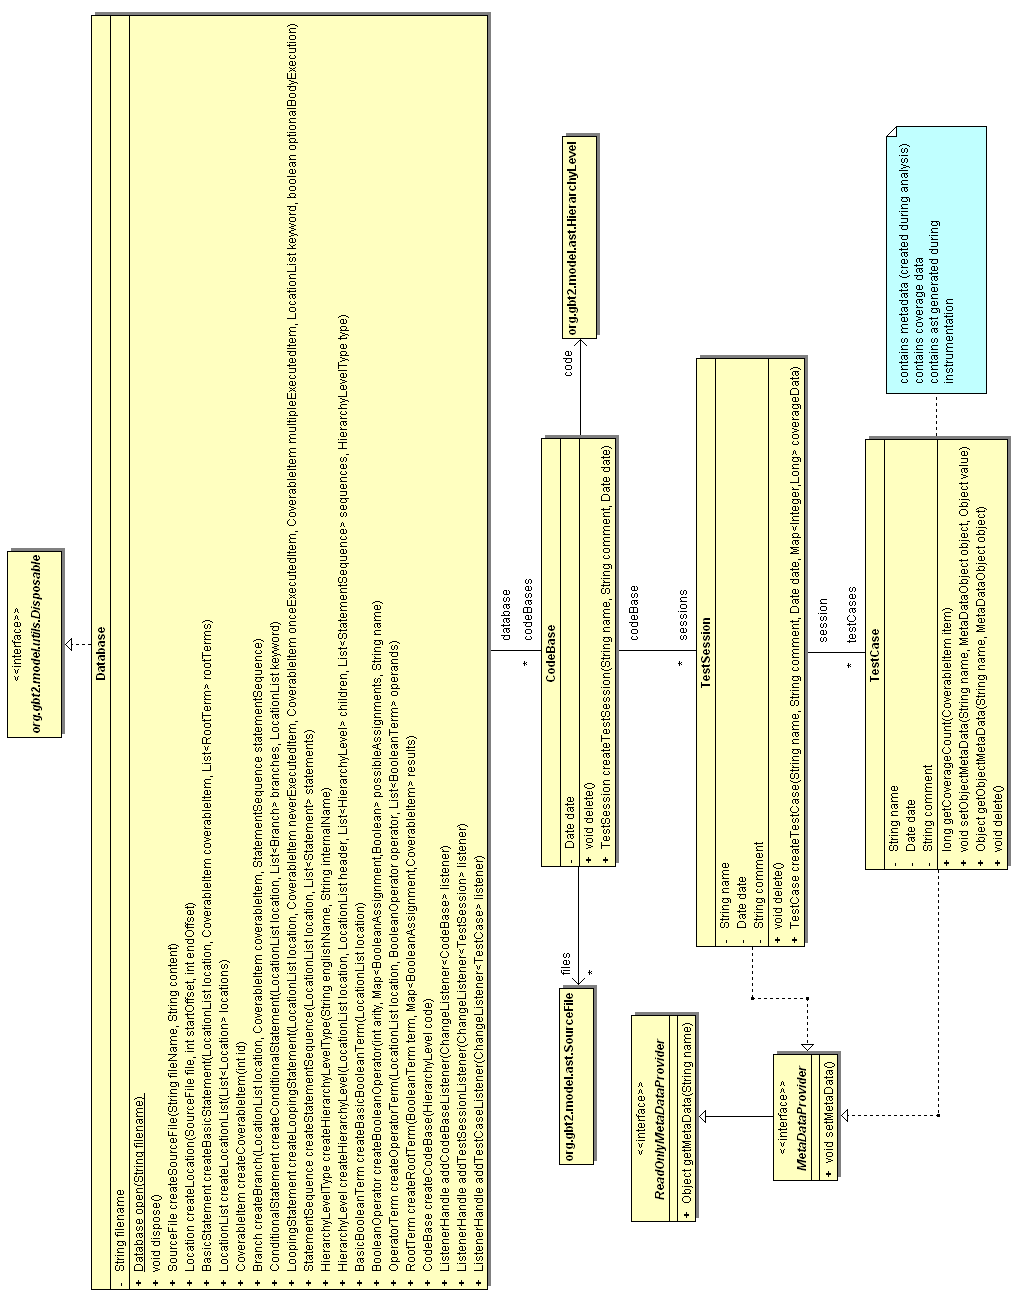
\includegraphics[width=1.0\textwidth]{images/Model/model_land.png}
 \caption{\pkg{\rootpkg.model}}
 \label{figure:Classes:Model}
\end{figure}

\subsubsection{\cls{Database}}

The class \cls{Database} represents a connection to a database.

This class is the central class in the data model; most other classes contain
a reference to this class.

A \obj{Database} contains references to the \obj{CodeBase}s.

The method \mtdst{open(...)} can be used with a filename to open the
connection.
The method \mtd{dispose()} can be used to close the connection.

\cls{Database} contains methods to create the AST objects.
(This methods are here
because the AST objects will contain a reference to the database connection.)

\mtd{createCodeBase(...)} can be used to create a code base with a given AST.

\mtd{addCodeBaseListener(...)}, \mtd{addTestSessionListener(...)} and
\mtd{addTestCaseListener(...)} will register a listener which will be called
if an object of the type \cls{CodeBase}, \cls{TestSession} or \cls{TestCase}
is changed.

\subsubsection{\cls{CodeBase}}

\cls{CodeBase} represents a code base.

It contains a reference to the AST, the date when the code base was created
and the \obj{TestSession}s which were created with this \obj{CodeBase}.

The method \mtd{delete()} can be used to delete the \obj{CodeBase} when
it has no \cls{TestSession}s.

The method \mtd{createTestSession(...)} can be used to create a new
\obj{TestSession}.

\subsubsection{\cls{TestSession}}

\cls{TestSession} represents a test session.

It contains a name, a comment, the date when the test session was created and
the \obj{TestCase}s belonging to this \obj{TestSession}.

The method \mtd{delete()} can be used to delete the \obj{TestSession} when
it has no \cls{TestCase}s.

The method \mtd{createTestCase(...)} can be used to create a new
\obj{TestCase}.

\subsubsection{\cls{TestCase}}

\cls{TestCase} represents a test case.

It contains a name, a comment, the date when the test case was created and
the coverage results.

The method \mtd{delete()} can be used to delete the \obj{TestCase}.

The method \mtd{getCoverageCount(...)} returns the coverage data for an
AST element.

The methods \mtd{setObjectMetaData(...)} and \mtd{getObjectMetaData(...)}
can set and get meta data for specific AST elements for this test case.
This meta data might be e.g. cached coverage metrics.

\subsubsection{\itf{MetaDataProvider}}

This interface is implemented by classes which allow to store additional meta
data (\cls{TestSession} and \cls{TestCase}).

This meta data might be e.g. the Eclipse project associated with a test
session.

\subsubsection{\itf{ReadOnlyMetaDataProvider}}

This interface is implemented by classes which allow a read only access to the
meta data stored into a \imp{MetaDataProvider}.

\subsubsection{Utils}
\namespace{\pkg{\rootpkg.model.utils}}

\begin{figure}[hbtp]
 \centering
 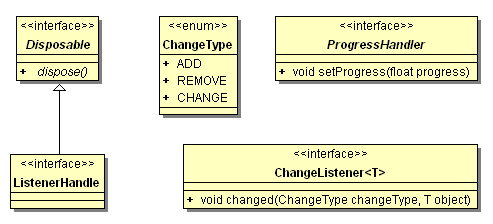
\includegraphics[width=0.7\textwidth]{images/Model/util.png}
 \caption{\pkg{\rootpkg.model.utils}}
 \label{figure:Classes:Model:Utils}
\end{figure}

\paragraph{\itf{Disposable}}

The \itf{Disposable} interface is implemented by all classes which contain
resources which have to be freed once the class istn't needed anymore.

For this purpose its only method \mtd{dispose()} should be called.

\paragraph{\itf{ListenerHandle}}

All methods in the data model which are used to register an event listener
return an instance implementing \itf{ListenerHandle}.

When \mtd{dispose()} ist called on this instance, the event listener will be
removed.

\paragraph{\cls{ChangeType}}

\cls{ChangeType} is an \code{enum} used to describe the type of a change event:

\begin{itemize}
\item[\code{ADD}]
  is used to describe that the object was added to its parent
\item[\code{REMOVE}]
  is used to describe that the object was removed from its parent
\item[\code{CHANGE}]
  is used to describe that some properties of the object were changed
\end{itemize}

\paragraph{\itf{ChangeListener<T>}}

The generic interface \itf{ChangeListener<T>} is to be implemented by classes
which want to listen
for change events for objects of type \code{T}.

The method \mtd{changed(...)} will be called with the \cls{ChangeType} and the
affected object each time a change occurs.

Implementors of this method have to be aware that this method will not
be called in the GUI thread.

\paragraph{\itf{ProgressHandler}}

\itf{ProgressHandler} should be implemented by classes which want to be
informed of the progress of an operation like a report generation or
an instrumentation.

In regular intervals the method \mtd{setProgess(...)} will be called with
a \code{float} between \code{0.0} and \code{1.0} representing a progess
between 0\% and 100\%.

Implementors of this method have to be aware that this method will not
be called in the GUI thread.

\subsubsection{AST}
\namespace{\pkg{\rootpkg.model.ast}}

\begin{figure}[hbtp]
 \centering
 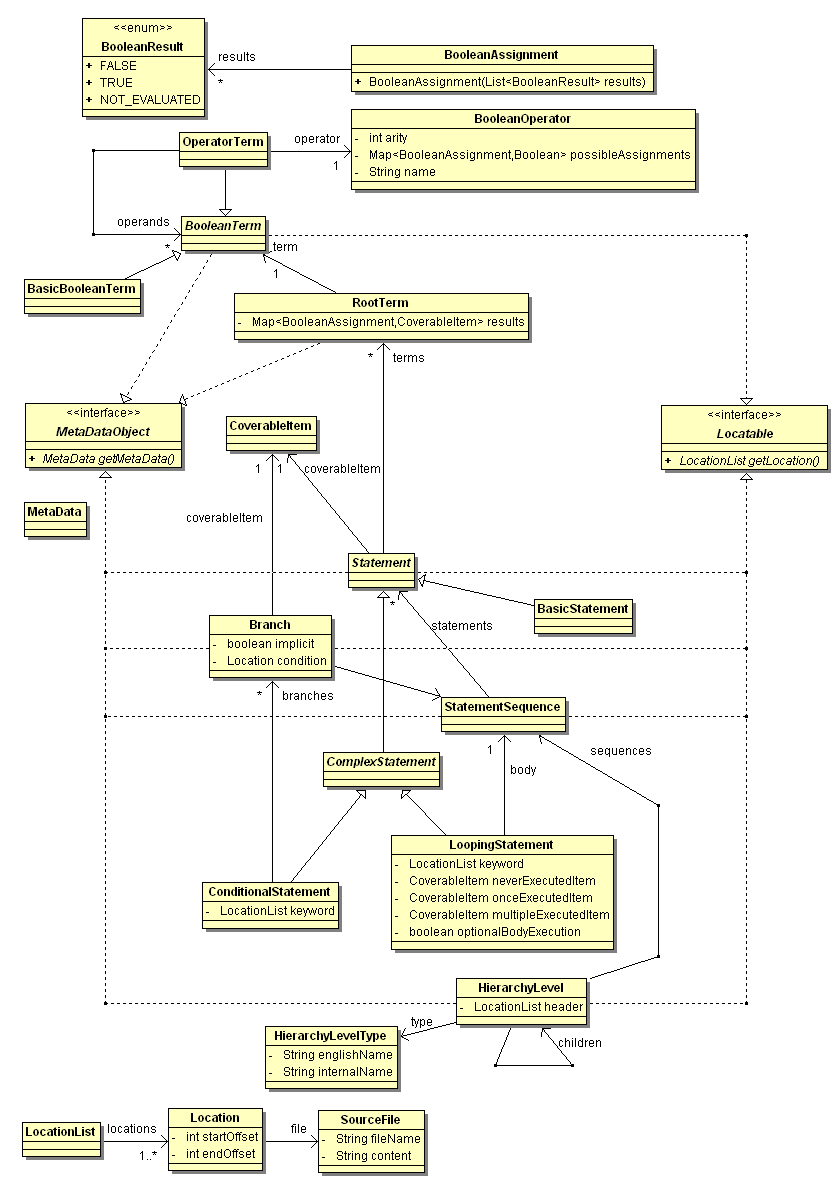
\includegraphics[width=1.0\textwidth]{images/Model/ast.png}
 \caption{\pkg{\rootpkg.model.ast}}
 \label{figure:Classes:Model:AST}
\end{figure}

\pkg{\rootpkg.model.ast} has classes to represent the abstract syntax tree
(AST) of the system under test.

\paragraph{\itf{MetaDataObject}}

\itf{MetaDataObject} is implemented by all classes to which meta data can be
associated.

It has only one method (\mtd{getMetaData()}) which can be used to get the
\cls{MetaData}.

Instances of this class can be passed to the methods
\mtd{setObjectMetaData(...)} and \mtd{getObjectMetaData(...)}
of the class \cls{TestCase}.

\paragraph{\cls{MetaData}}

A \obj{MetaData} represents the meta data associated to a AST element.

This class is used internally.

\paragraph{\cls{CoverableItem}}

A \obj{CoverableItem} represents a coverable item which can be covered in
a test case.

Instances of this class can be passed to the method \mtd{getCoverageCount(...)}
of the class \cls{TestCase}.

\paragraph{\itf{Locatable}}

A \imp{Locatable} is an object with one or multiple locations.

The method \mtd{getLocation()} can be used to get this locations.

\paragraph{\cls{LocationList}}

A \obj{LocationList} is a list of \obj{Location}s.

This is necessary since some AST elements can have mulitple locations
(e.g. a \code{partial class} in C\#).

\paragraph{\cls{Location}}

A \obj{Location} is a segment in a code file.

It is given by its \fld{startOffset} (which is the offset of the
first \code{char} belonging to the location), its \fld{endOffset}
(which is the offset of the first \code{char} no longer belonging to the
location), and the file which contains this location.

\paragraph{\cls{SourceFile}}

A \cls{SourceFile} represents a source file.

It contains the \fld{fileName} and the \fld{content} of the file.

\paragraph{\cls{BooleanResult}}

A \obj{BooleanResult} is an \code{enum} which describes the result of the
evaluation of a boolean term.

The value \code{NOT\_EVALUATED} is used if a subterm was not evaluated, e.g.
because of the short circuit behaviour of an operator.

\paragraph{\cls{BooleanAssignment}}

A \obj{BooleanAssignment} assigns every basic boolean term of a boolean term
an \obj{BooleanResult}.

\paragraph{\clsab{BooleanTerm}}

A \obj{BooleanTerm} represents a boolean term which ist constructed of basic
boolean terms and boolean operators.

A \obj{BooleanTerm} can be a \cls{BasicBooleanTerm} or a \cls{OperatorTerm}.

\paragraph{\cls{BasicBooleanTerm}}

A \obj{BasicBooleanTerm} represents a basic boolean term which is considered
atomic.

\paragraph{\cls{OperatorTerm}}

A \obj{OperatorTerm} represents a boolean term which consists of an operator
connect zero, one or more \obj{BooleanTerm}s.

It contains a reference to the \obj{BooleanOperator} used and the list of the
operands (which are \obj{BooleanTerm}s).

\paragraph{\cls{BooleanOperator}}

A \obj{BooleanOperator} is a function with a given arity \fld{arity} which maps
a \fld{arity}-tuple of boolean values to a boolean value.

The object contains the \fld{arity}, a map which maps the assignments to the
result and a \fld{name}.

\paragraph{\cls{RootTerm}}

A \obj{RootTerm} is a boolean term which is not a part of another boolean term.

A \obj{RootTerm} consists of a \obj{BooleanTerm} and a \obj{CoverableItem}
for every possible assignment of this term.

\paragraph{\clsab{Statement}}

A \obj{Statement} is a basic or a complex statement.

Every \obj{Statement} either has the type \cls{BasicStatement} or on of
the types derived of \cls{ComplexStatement}, \cls{ConditionalStatement} and
\cls{LoopingStatement}.

A \obj{Statement} has a list of \obj{RootTerm}s which appear in the statement
and a \obj{CoverableItem} which will be covered when the \obj{Statement}
is executed.

\paragraph{\cls{BasicStatement}}

A \obj{BasicStatement} is a statement which contains no other statements.

\paragraph{\clsab{ComplexStatement}}

A \obj{ComplexStatement} is a statement which can contain other statements and
is either a \obj{ConditionalStatement} or a \obj{LoopingStatement}.

\paragraph{\cls{ConditionalStatement}}

A \obj{ConditionalStatement} is a statement where the control flow splits up
into a number of \obj{Branch}es.

The \obj{ConditionalStatement} consists of these \obj{Branch}es and of the
\obj{LocationList} of the keyword of the statement (for the purpose of
coloring the source code). %% TODO: American vs. British English?

\paragraph{\cls{Branch}}

A \obj{Branch} is a branch which can be taken in a conditonal statement.

It consists of a \obj{StatementSequence},
a \obj{CoverableItem} which is covered when the branch
is executed, a flag which says that this branch does not appear explicitly
in the source code (e.g. a \code{else} branch when there is no \code{else}
keyword for a \code{if} statement or the \code{default} branch of a
\code{select} statement where there is no \code{default:} block) and 
optionally the \obj{LocationList} of the conditon whether this branch is taken
(for the purpose of coloring the source code).

\paragraph{\cls{LoopingStatement}}

A \obj{LoopingStatement} is a statement which has a body which can be executed
a number of times not known at compile time.

It has a \obj{StatementSequence} representing the body, the \obj{LocationList}
of the keyword of the statement (for the purpose of coloring the source code),
a boolean flag indicating whether the body also can be executed zero times
and three \obj{CoverableItem}s covered when the body is executed zero times,
one time or more often.

\paragraph{\cls{StatementSequence}}

A \obj{StatementSequence} is a list of \obj{Statement}s.

\subsection{Instrumentation} \label{Instrumentation}

\namespace{\pkg{\rootpkg.instrumentation}}

\subsubsection{General procedure}

\begin{figure}[hbtp]
 \centering
 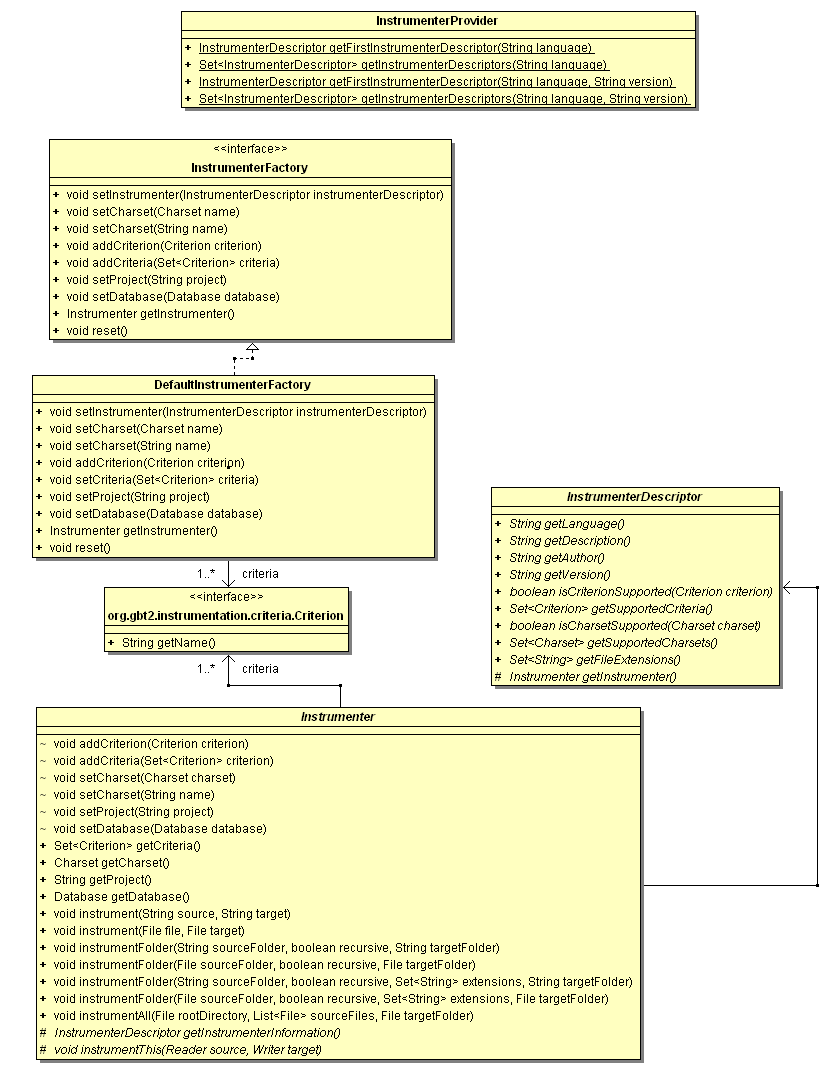
\includegraphics[width=0.9\textwidth]{images/instrumentation/instrumentation.png}
 \caption{\pkg{\rootpkg.instrumentation}}
 \label{figure:Classes:Instrumentation}
\end{figure}

\par This section describes how the classes in \pkg{\rootpkg.instrumentation} can be used to instrument a source file. \sloppy \par The first step is to get an \clsab{InstrumenterDescriptor} for the respective programming language the source file is written in. This \obj{InstrumenterDescriptor} can be obtained by passing the name of the programming language either to \cls{InstrumenterProvider.}\mtdst{getFirstInstrumenterDescriptor(...)} or \cls{InstrumenterProvider.}\mtdst{getInstrumenterDescriptors(...)}, to get the first available instrumenter or a list of all instrumenters which are available for the programming language. \fussy \par \clsab{InstrumenterDescriptor} offers several methods to get detailed information about the corresponding \clsab{Instrumenter}, e.g. supported charsets, description, author or version information. \clsab{InstrumenterDescriptor.}\mtd{getSupportedCriteria(...)} returns a list of criteria which are supported by the corresponding \clsab{Instrumenter}.
\par The desired criteria are chosen from this list. To create an actual instance of \clsab{Instrumenter} a factory is used. A factory needs to implement at least the methods defined in \itf{InstrumenterFactory}, a default implementation is offered by \cls{DefaultInstrumenterFactory}. \itf{InstrumenterFactory.}\mtd{setInstrumenter(...)} receives the previously obtained \clsab{InstrumenterDescriptor} and \itf{InstrumenterFactory.}\mtd{addCriterion(...)} is called for every \itf{Criterion} which was selected from the \clsab{InstrumenterDescriptor}. In the same way the desired charset can be set. \par To get an instance of \clsab{Instrumenter} with the desired properties passed to the factory, \itf{InstrumenterFactory.}\mtd{getInstrumenter()} needs to be called. \par To use the newly created \obj{Instrumenter} on a source file or folder containing source files, \clsab{Instrumenter.}\mtd{instrument(...)} or \clsab{Instrumenter.}\mtd{instrumentFolder(...)} can be used.
\par In order to add another instrumenter you simply create a subclass of \clsab{Instrumenter} with the desired functionality and a corresponding \clsab{InstrumenterDescriptor}. With the help of reflection this new instrumenter will be available through the \cls{InstrumenterProvider} (under the assumption that the necessary files are at a certain place, the exact location for new instrumenters will be determined during implementation).
%%%%%%%%%%%%%%%%%%%%%%%%%%%%%%%%%%%%%%%%%%%%%%%%%%%%%%%%%%
% InstrumenterProvider
%%%%%%%%%%%%%%%%%%%%%%%%%%%%%%%%%%%%%%%%%%%%%%%%%%%%%%%%%%
\subsubsection{\cls{InstrumenterProvider}} \label{Classes:Instrumentation:InstrumenterProvider}
\namespace{\pkg{\rootpkg.instrumentation.}\cls{InstrumenterProvider}}

This class is used to get descriptions of instrumenters which target a certain programming language.

\paragraph{\mtdst{getFirstInstrumenterDescriptor(language)}} \label{Classes:Instrumentation:InstrumenterProvider:getFirstInstrumenterDescriptor}
The parameters of this method are:
\begin{description}
\item[language:] The target language of the instrumenter as a \cls{String}, e.g. ``java''.

\end{description}
This method returns an \obj{InstrumenterDescriptor} for the desired target language.

\paragraph{\mtdst{getInstrumenterDescriptors(language)}} \label{Classes:Instrumentation:InstrumenterProvider:getInstrumenterDescriptors_language}
The parameters of this method are:
\begin{description}
\item[language:] The target language of the instrumenter as a \cls{String}, e.g. ``java''.

\end{description}
This method returns a set of \obj{InstrumenterDescriptor}, with each of them targetting the passed language.

\paragraph{\mtdst{getFirstInstrumenterDescriptor(language, version)}} \label{Classes:Instrumentation:InstrumenterProvider:getFirstInstrumenterDescriptor_version}
The parameters of this method are:
\begin{description}
\item[language:] The target language of the instrumenter as a \cls{String}, e.g. ``java''.
\item[version:] The version of the target language as a \cls{String}, e.g. ``1.5''.

\end{description}
This method returns an \obj{InstrumenterDescriptor} for the desired target language.

\paragraph{\mtdst{getInstrumenterDescriptors(language, version)}} \label{Classes:Instrumentation:InstrumenterProvider:getInstrumenterDescriptors_language_version}
The parameters of this method are:
\begin{description}
\item[language:] The target language of the instrumenter as a \cls{String}, e.g. ``java''.
\item[version:] The version of the target language as a \cls{String}, e.g. ``1.5''.

\end{description}
This method returns a set of \obj{InstrumenterDescriptor}, with each of them targetting the passed language.

%%%%%%%%%%%%%%%%%%%%%%%%%%%%%%%%%%%%%%%%%%%%%%%%%%%%%%%%%%
% Criterion
%%%%%%%%%%%%%%%%%%%%%%%%%%%%%%%%%%%%%%%%%%%%%%%%%%%%%%%%%%
\subsubsection{\itf{Criterion}} \label{Classes:Instrumentation:Criterion}
\namespace{\pkg{\rootpkg.instrumentation.criteria.}\itf{Criterion}}

This interface gives access to certain information about a particular coverage criterion.

\paragraph{\mtd{getName()}} \label{Classes:Instrumentation:Criterion:getName}
This method returns the name of the coverage criterion as a \cls{String}, e.g. ``statement-coverage''.

%%%%%%%%%%%%%%%%%%%%%%%%%%%%%%%%%%%%%%%%%%%%%%%%%%%%%%%%%%
% InstrumenterDescriptor
%%%%%%%%%%%%%%%%%%%%%%%%%%%%%%%%%%%%%%%%%%%%%%%%%%%%%%%%%%
\subsubsection{\clsab{InstrumenterDescriptor}} \label{Classes:Instrumentation:InstrumenterDescriptor}
\namespace{\pkg{\rootpkg.instrumentation.}\clsab{InstrumenterDescriptor}}

This interface gives access to certain information about a particular instrumenter.

\paragraph{\mtd{getLanguage()}} \label{Classes:Instrumentation:InstrumenterDescriptor:getLanguage}
This method returns the  target language of the instrumenter as a \cls{String}, e.g. ``java''.
\paragraph{\mtd{getDescription()}} \label{Classes:Instrumentation:InstrumenterDescriptor:getDescription}
This method returns the description of the instrumenter as a \cls{String}.
\paragraph{\mtd{getAuthor()}} \label{Classes:Instrumentation:InstrumenterDescriptor:getAuthor}
This method returns the name of the author of the instrumenter as a \cls{String}.
\paragraph{\mtd{getVersion()}} \label{Classes:Instrumentation:InstrumenterDescriptor:getVersion}
This method returns the version information of the instrumenter as a \cls{String}.
\paragraph{\mtd{isCriterionSupported(criterion)}} \label{Classes:Instrumentation:InstrumenterDescriptor:isCriterionSupported}
The parameters of this method are:
\begin{description}
\item[criterion:] The \imp{Criterion} to check for.

\end{description}
This method returns true if the passed \imp{Criterion} is supported by the instrumenter, false if not.
\paragraph{\mtd{getSupportedCriteria()}} \label{Classes:Instrumentation:InstrumenterDescriptor:getSupportedCriteria}
This method returns a set of \imp{Criterion} which are supported by the instrumenter belonging to this \obj{InstrumenterDescriptor}.
\paragraph{\mtd{isCharsetSupported(charset)}} \label{Classes:Instrumentation:InstrumenterDescriptor:isCharsetSupported}
The parameters of this method are:
\begin{description}
\item[charset:] The \obj{Charset} to check for.

\end{description}
This method returns true if the passed \obj{Charset} is supported by the instrumenter, false if not.
\paragraph{\mtd{getSupportedCharset()}} \label{Classes:Instrumentation:InstrumenterDescriptor:getSupportedCharsets}
This method returns a set of \obj{Charset} which are supported by the instrumenter belonging to this \obj{InstrumenterDescriptor}.
\paragraph{\mtd{getFileExtensions()}} \label{Classes:Instrumentation:InstrumenterDescriptor:getFileExtensions}
This method returns a set of file extensions of source files which are supported by the instrumenter belonging to this \obj{InstrumenterDescriptor}.
\paragraph{\mtd{getInstrumenter()}} \label{Classes:Instrumentation:InstrumenterDescriptor:getInstrumenter}
This method returns the \obj{Instrumenter} which belongs to the \obj{InstrumenterDescriptor}, it should only be called from a \imp{InstrumenterFactory}.

%%%%%%%%%%%%%%%%%%%%%%%%%%%%%%%%%%%%%%%%%%%%%%%%%%%%%%%%%%
% InstrumenterFactory
%%%%%%%%%%%%%%%%%%%%%%%%%%%%%%%%%%%%%%%%%%%%%%%%%%%%%%%%%%
\subsubsection{\itf{InstrumenterFactory}} \label{Classes:Instrumentation:InstrumenterFactory}
\namespace{\pkg{\rootpkg.instrumentation.}\itf{InstrumenterFactory}}

This interface needs to be implemented by a class which wants to act as a factory for \obj{Instrumenter}.

\paragraph{\mtd{setInstrumenter(instrumenterDescriptor)}} \label{Classes:Instrumentation:InstrumenterFactory:setInstrumenter}
The parameters of this method are:
\begin{description}
\item[instrumenterDescriptor:] The \obj{InstrumenterDescriptor}, whose corresponding \obj{Instrumenter} to create.
\end{description}
\paragraph{\mtd{setCharset(charset)}} \label{Classes:Instrumentation:InstrumenterFactory:setCharset}
The parameters of this method are:
\begin{description}
\item[charset:] The \obj{Charset}, to use when reading source files.
\end{description}
\paragraph{\mtd{setCharset(charsetName)}} \label{Classes:Instrumentation:InstrumenterFactory:setCharset_name}
The parameters of this method are:
\begin{description}
\item[charsetName:] The name of a \cls{Charset} as a \cls{String}, which is used when reading source files.
\end{description}
\paragraph{\mtd{addCriterion(criterion)}} \label{Classes:Instrumentation:InstrumenterFactory:addCriterion}
The parameters of this method are:
\begin{description}
\item[criterion:] The \imp{Criterion} the instrumenter should support, valid criteria can be obtained by calling \clsab{InstrumenterDescriptor.}\mtd{getSupportedCriteria()} of the corresponding \obj{InstrumenterDescriptor}.
\end{description}
\paragraph{\mtd{addCriteria(criteria)}} \label{Classes:Instrumentation:InstrumenterFactory:addCriteria}
The parameters of this method are:
\begin{description}
\item[criteria:] A set of \imp{Criterion} the instrumenter should support, valid criteria can be obtained by calling \clsab{InstrumenterDescriptor.}\mtd{getSupportedCriteria()} of the corresponding \obj{InstrumenterDescriptor}.
\end{description}
\paragraph{\mtd{setProject(project)}} \label{Classes:Instrumentation:InstrumenterFactory:setProject}
The parameters of this method are:
\begin{description}
\item[project:] The Eclipse project to whom the \obj{Instrumenter} should belong to. The exact type of this reference will be chosen during implementation.
\end{description}
\paragraph{\mtd{setDatabase(database)}} \label{Classes:Instrumentation:InstrumenterFactory:setDatabase}
The parameters of this method are:
\begin{description}
\item[database:] The \obj{Database} to whom the \obj{Instrumenter} should belong to.
\end{description}
\paragraph{\mtd{reset()}} \label{Classes:Instrumentation:InstrumenterFactory:reset}
This method resets the factory, all fields need to bet set again.
\paragraph{\mtd{getInstrumenter()}} \label{Classes:Instrumentation:InstrumenterFactory:getInstrumenter}
This method returns the \obj{Instrumenter} which belongs to the \obj{InstrumenterDescriptor}, taking into account the specified \obj{Charset} and list of \imp{Criterion}.

%%%%%%%%%%%%%%%%%%%%%%%%%%%%%%%%%%%%%%%%%%%%%%%%%%%%%%%%%%
% DefaultInstrumenterFactory
%%%%%%%%%%%%%%%%%%%%%%%%%%%%%%%%%%%%%%%%%%%%%%%%%%%%%%%%%%
\subsubsection{\cls{DefaultInstrumenterFactory}} \label{Classes:Instrumentation:DefaultInstrumenterFactory}
\namespace{\pkg{\rootpkg.instrumentation.}\cls{DefaultInstrumenterFactory}}

A default implementation of \itf{InstrumenterFactory}

\paragraph{\mtd{setInstrumenter(instrumenterDescriptor)}} \label{Classes:Instrumentation:DefaultInstrumenterFactory:setInstrumenter}
The parameters of this method are:
\begin{description}
\item[instrumenterDescriptor:] The \obj{InstrumenterDescriptor}, whose corresponding \obj{Instrumenter} to create.
\end{description}
\paragraph{\mtd{setCharset(charset)}} \label{Classes:Instrumentation:DefaultInstrumenterFactory:setCharset}
The parameters of this method are:
\begin{description}
\item[charset:] The \obj{Charset}, to use when reading source files.
\end{description}
\paragraph{\mtd{setCharset(charsetName)}} \label{Classes:Instrumentation:DefaultInstrumenterFactory:setCharset_name}
The parameters of this method are:
\begin{description}
\item[charsetName:] The name of a \cls{Charset} as a \cls{String}, which is used when reading source files.
\end{description}
\paragraph{\mtd{addCriterion(criterion)}} \label{Classes:Instrumentation:DefaultInstrumenterFactory:addCriterion}
The parameters of this method are:
\begin{description}
\item[criterion:] The \imp{Criterion} the instrumenter should support, valid criteria can be obtained by calling \clsab{InstrumenterDescriptor.}\mtd{getSupportedCriteria()} of the corresponding \obj{InstrumenterDescriptor}.
\end{description}
\paragraph{\mtd{addCriteria(criteria)}} \label{Classes:Instrumentation:DefaultInstrumenterFactory:addCriteria}
The parameters of this method are:
\begin{description}
\item[criteria:] A set of \imp{Criterion} the instrumenter should support, valid criteria can be obtained by calling \clsab{InstrumenterDescriptor.}\mtd{getSupportedCriteria()} of the corresponding \obj{InstrumenterDescriptor}.
\end{description}
\paragraph{\mtd{setProject(project)}} \label{Classes:Instrumentation:DefaultInstrumenterFactory:setProject}
The parameters of this method are:
\begin{description}
\item[project:] The Eclipse project to whom the \obj{Instrumenter} should belong to. The exact type of this reference will be chosen during implementation.
\end{description}
\paragraph{\mtd{setDatabase(database)}} \label{Classes:Instrumentation:DefaultInstrumenterFactory:setDatabase}
The parameters of this method are:
\begin{description}
\item[database:] The \obj{Database} to whom the \obj{Instrumenter} should belong to.
\end{description}
\paragraph{\mtd{reset()}} \label{Classes:Instrumentation:DefaultInstrumenterFactory:reset}
This method resets the factory, all fields need to bet set again.
\paragraph{\mtd{getInstrumenter()}} \label{Classes:Instrumentation:DefaultInstrumenterFactory:getInstrumenter}
This method returns the \obj{Instrumenter} which belongs to the \obj{InstrumenterDescriptor}, taking into account the specified \obj{Charset} and list of \imp{Criterion}.

%%%%%%%%%%%%%%%%%%%%%%%%%%%%%%%%%%%%%%%%%%%%%%%%%%%%%%%%%%
% Instrumenter
%%%%%%%%%%%%%%%%%%%%%%%%%%%%%%%%%%%%%%%%%%%%%%%%%%%%%%%%%%
\subsubsection{\clsab{Instrumenter}} \label{Classes:Instrumentation:Instrumenter}
\namespace{\pkg{\rootpkg.instrumentation.}\clsab{Instrumenter}}

This is the abstract class every instrumenter needs to be derived from. It offers utility methods for easy traversal of directory trees.
\paragraph{\mtd{getCriteria()}} \label{Classes:Instrumentation:Instrumenter:getCriteria}
This method returns a set of \imp{Criterion} which are supported by the \obj{Instrumenter}.
\paragraph{\mtd{getCharset()}} \label{Classes:Instrumentation:Instrumenter:getCharset}
This method returns the \obj{Charset} which is used when reading source files.
\paragraph{\mtd{getProject()}} \label{Classes:Instrumentation:Instrumenter:getProject}
This method returns a reference to the Eclipse project to whom the \obj{Instrumenter} belongs to. The exact type of this reference will be chosen during implementation.
\paragraph{\mtd{getDatabase()}} \label{Classes:Instrumentation:Instrumenter:getDatabase}
This method returns the \obj{Database} which is used by the \obj{Instrumenter} to store static data which is generated during instrumentation.
\paragraph{\mtd{instrument(source, target)}} \label{Classes:Instrumentation:Instrumenter:instrument}
The parameters of this method are:
\begin{description}
\item[source:] The path to the source file to instrument as a \obj{String}.
\item[target:] The path to the file which will contain the instrumented version of the source file as a \obj{String}.
\end{description}
\paragraph{\mtd{instrument(sourceFile, targetFile)}} \label{Classes:Instrumentation:Instrumenter:instrument_file}
The parameters of this method are:
\begin{description}
\item[sourceFile:] The source \obj{File} to instrument.
\item[targetFile:] The path to the \obj{File} which will contain the instrumented version of the source \obj{File}.
\end{description}
\paragraph{\mtd{instrumentFolder(sourceFolder, recursive, targetFolder)}} \label{Classes:Instrumentation:Instrumenter:instrumentFolder}
The parameters of this method are:
\begin{description}
\item[sourceFolder:] The path to the folder which contains source files to instrument.
\item[recursive:] A flag to denote whether the source folder should be traversed recursively.
\item[targetFolder:] The path to the folder which will contain the instrumented versions of the source files.
\end{description}
\paragraph{\mtd{instrumentFolder(sourceFolder, recursive, targetFolder)}} \label{Classes:Instrumentation:Instrumenter:instrumentFolder_file}
The parameters of this method are:
\begin{description}
\item[sourceFolder:] The folder as a \obj{File} which contains source files to instrument.
\item[recursive:] A flag to denote whether the source folder should be traversed recursively.
\item[targetFolder:] The folder which will contain the instrumented versions of the source files as a \obj{File}.
\end{description}
\paragraph{\mtd{instrumentFolder(sourceFolder, recursive, extensions, targetFolder)}} \label{Classes:Instrumentation:Instrumenter:instrumentFolder_ext}
The parameters of this method are:
\begin{description}
\item[sourceFolder:] The path to the folder which contains source files to instrument.
\item[recursive:] A flag to denote whether the source folder should be traversed recursively.
\item[extensions:] A set of valid file extensions of source files which can be instrumented.
\item[targetFolder:] The path to the folder which will contain the instrumented versions of the source files.
\end{description}
\paragraph{\mtd{instrumentFolder(sourceFolder, recursive, extensions, targetFolder)}} \label{Classes:Instrumentation:Instrumenter:instrumentFolder_ext_file}
The parameters of this method are:
\begin{description}
\item[sourceFolder:] The folder as a \obj{File} which contains source files to instrument.
\item[recursive:] A flag to denote whether the source folder should be traversed recursively.
\item[extensions:] A set of valid file extensions of source files which can be instrumented.
\item[targetFolder:] The folder which will contain the instrumented versions of the source files as a \obj{File}.
\end{description}
\paragraph{\mtd{instrumentAll(rootDirectory, sourceFiles, targetFolder)}} \label{Classes:Instrumentation:Instrumenter:instrumentAll}
The parameters of this method are:
\begin{description}
\item[rootDirectory:] The folder as a \obj{File} which contains source files to instrument, either directly or indirectly through subfolders.
\item[sourceFiles:] A list of \obj{File} which should be instrumented, they need to be relative to the rootDirectory.
\item[targetFolder:] The folder which will contain the instrumented versions of the source files as a \obj{File}.
\end{description}




%%%%%%%%%%%%%%%%%%%%%%%%%%%%%%%%%%%%%%%%%%%%%%%%%%%%%%%%%%
%%%%%%%%%%%%%%%%%%%%%%%%%%%%%%%%%%%%%%%%%%%%%%%%%%%%%%%%%%
% Metrics
%%%%%%%%%%%%%%%%%%%%%%%%%%%%%%%%%%%%%%%%%%%%%%%%%%%%%%%%%%
\subsection{Metrics}
\namespace{\pkg{\rootpkg.metrics}}

\begin{figure}[hbtp]
 \centering
 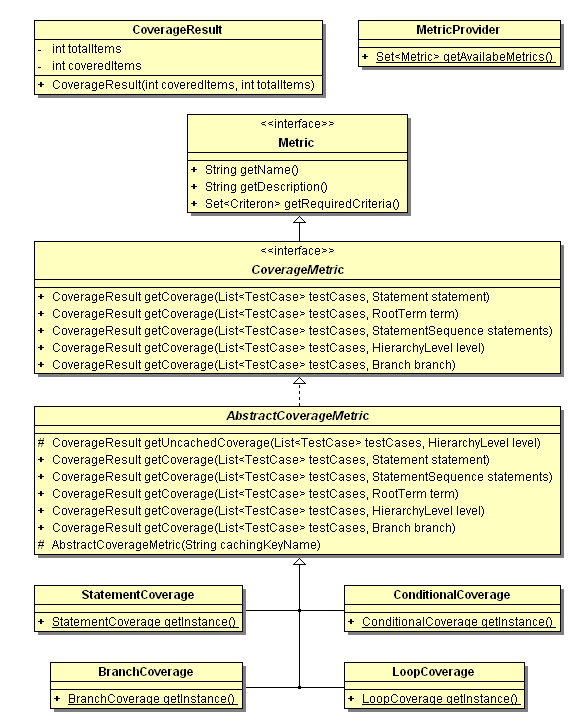
\includegraphics[height=0.8\textheight]{images/Metrics/metrics.png}
 \caption{\pkg{\rootpkg.metrics}}
 \label{figure:Classes:Metrics:metrics}
\end{figure}

%%%%%%%%%%%%%%%%%%%%%%%%%%%%%%%%%%%%%%%%%%%%%%%%%%%%%%%%%%
% General procedure
%%%%%%%%%%%%%%%%%%%%%%%%%%%%%%%%%%%%%%%%%%%%%%%%%%%%%%%%%%
\subsubsection{General procedure} % to perform an analysis
This section describes how the classes in \pkg{\rootpkg.metrics} can be used to acquire the coverage of certain test cases in regards to certain parts of the source code. The first step is to get an instance of the class implementing the coverage metric one wants to calculate. This can be achieved by either calling the \cls{MetricProvider.}\mtdst{getAvailableMetrics}, to obtain a list of all classes that implement \itf{Metric}, or by calling \mtdst{getInstance()} of the class itself. Now one calls \mtd{getCoverage(...)} with the test cases and the parts of the AST one wishes to examine. The returned \cls{CoverageResult} contains the coverage measured by the test cases in regards to the parts of the AST given.

%%%%%%%%%%%%%%%%%%%%%%%%%%%%%%%%%%%%%%%%%%%%%%%%%%%%%%%%%%
% CoverageResult
%%%%%%%%%%%%%%%%%%%%%%%%%%%%%%%%%%%%%%%%%%%%%%%%%%%%%%%%%%
\subsubsection{\cls{CoverageResult}} \label{Classes:Metrics:CoverageResult}
\namespace{\pkg{\rootpkg.metrics.}\cls{CoverageResult}}

This class is used to store the results calculated during the analysis of coverable items.

\paragraph{\mtd{CoverageResult(coveredItems, totalItems)}} \label{Classes:Metrics:CoverageResult:CoverageResult}
The parameters of this method are:
\begin{description}
\item[coveredItems:] The number of covered coverable items examined during the computation of the coverage. Is always smaller or equal to the total number of  coverable items.

\item[totalItems:] The total number of all coverable items examined during the computation of the coverage.

\end{description}

%%%%%%%%%%%%%%%%%%%%%%%%%%%%%%%%%%%%%%%%%%%%%%%%%%%%%%%%%%
% Metric
%%%%%%%%%%%%%%%%%%%%%%%%%%%%%%%%%%%%%%%%%%%%%%%%%%%%%%%%%%
\subsubsection{\itf{Metric}} \label{Classes:Metrics:Metric}
\namespace{\pkg{\rootpkg.metrics.}\itf{Metric}}

This interface should be implemented by all classes, that are used to analyze parts of the data model.

\paragraph{\mtd{getName()}} \label{Classes:Metrics:Metric:getName}

Every metric has a unique name, that can be used to differeniate between metrics.

\paragraph{\mtd{getDescription()}} \label{Classes:Metrics:Metric:getDescription}

Every metric has a description, that explains the purpose of the metric.

\paragraph{\mtd{getRequiredCriteria()}} \label{Classes:Metrics:Metric:getRequiredCriteria}

The returned set of \itf{Criterion} denotes the criteria that had to have been used during the instrumentation process. E.g. to calculate the statement coverage of a test run of a SUT, said SUT must have been instrumented to calculate statement coverage. It is only sensible to apply a \itf{Metric} if its required criteria are a subset of the criteria used in the instrumentation process.

%%%%%%%%%%%%%%%%%%%%%%%%%%%%%%%%%%%%%%%%%%%%%%%%%%%%%%%%%%
% MetricsProvider
%%%%%%%%%%%%%%%%%%%%%%%%%%%%%%%%%%%%%%%%%%%%%%%%%%%%%%%%%%
\subsubsection{\cls{MetricProvider}} \label{Classes:Metrics:MetricProvider}
\namespace{\pkg{\rootpkg.metrics.}\cls{MetricProvider}}

This class is used to get an instance of all classes, that implement \itf{Metric}.

\paragraph{\mtdst{getAvailableMetrics()}} \label{Classes:Metrics:MetricProvider:getAvailableMetrics}
This method returns a list of the instances of all classes, that implement \itf{Metric}. This is done through reflection.

%%%%%%%%%%%%%%%%%%%%%%%%%%%%%%%%%%%%%%%%%%%%%%%%%%%%%%%%%%
% CoverageMetric
%%%%%%%%%%%%%%%%%%%%%%%%%%%%%%%%%%%%%%%%%%%%%%%%%%%%%%%%%%
\subsubsection{\itf{CoverageMetric}} \label{Classes:Metrics:CoverageMetric}
\namespace{\pkg{\rootpkg.metrics.}\itf{CoverageMetric}}
This interface is intented to be implemented by all coverage metrics.

\paragraph{\mtd{getCoverage(testCases, level)}} \label{Classes:Metrics:CoverageMetric:getCoverage_hierarchy}
The parameters of this method are:
\begin{description}
\item[testCases:] The list containing \cls{TestCase}s, whose combined coverage is calculated here.

\item[level:]  The \cls{HierarchyLevel} which is the entry point into the AST.

\end{description}

\paragraph{\mtd{getCoverage(testCases, statements)}} \label{Classes:Metrics:CoverageMetric:getCoverage_statements}
The parameters of this method are:
\begin{description}
\item[testCases:] The list containing \cls{TestCase}s, whose combined coverage is calculated here.

\item[statements:] The \cls{StatementSequence} which contains the statements whose coverage is to be calculated.

\end{description}

\paragraph{\mtd{getCoverage(testCases, statement)}} \label{Classes:Metrics:CoverageMetric:getCoverage_statement}
The parameters of this method are:
\begin{description}
\item[testCases:] The list containing \cls{TestCase}s, whose combined coverage is calculated here.

\item[statement:]  The \clsab{Statement} whose coverage is to be calculated.

\end{description}

\paragraph{\mtd{getCoverage(testCases, branch)}} \label{Classes:Metrics:CoverageMetric:getCoverage_branch}
The parameters of this method are:
\begin{description}
\item[testCases:] The list containing \cls{TestCase}s, whose combined coverage is calculated here.

\item[branch:] The \cls{Branch} whose coverage is to be calculated.

\end{description}

\paragraph{\mtd{getCoverage(testCases, term)}} \label{Classes:Metrics:CoverageMetric:getCoverage_term}
The parameters of this method are:
\begin{description}
\item[testCases:] The list containing \cls{TestCase}s, whose combined coverage is calculated here.

\item[term:]  The \clsab{RootTerm} whose coverage is to be calculated.

\end{description}

%%%%%%%%%%%%%%%%%%%%%%%%%%%%%%%%%%%%%%%%%%%%%%%%%%%%%%%%%%
% AbstractCoverageMetric
%%%%%%%%%%%%%%%%%%%%%%%%%%%%%%%%%%%%%%%%%%%%%%%%%%%%%%%%%%
\subsubsection{\clsab{AbstractCoverageMetric}} \label{Classes:Metrics:AbstractCoverageMetric}
\namespace{\pkg{\rootpkg.metrics.}\clsab{AbstractCoverageMetric}}
This abstract class implements the \itf{CoverageMetric}. It provides a default implementation for all methods declared in \itf{CoverageMetric}. Classes subclassing \clsab{AbstractCoverageMetric} need only override those methods, whose implementation here differs from behaviour they require. It also provides caching functionality for the coverage results calculated for \cls{HierarchyLevel}s. Every calculation done solely with the methods of this class will always return zero coverage. But they provide a way to traverse the AST. To implement e.g. statement coverage, it would be necessary to override \mtd{getCoverage(testCases, statement)} and check, if a basic statement is given and return the true coverage. But for the traversal of the AST one can call \cls{super.}\mtd{getCoverage(testCases, statement)}. 

\paragraph{\mtd{getCoverage(testCases, level)}} \label{Classes:Metrics:AbstractCoverageMetric:getCoverage_hierarchy}
This method first checks, if the coverage of the given \cls{TestCase}s and the given \cls{HierarchyLevel} has been calculated and stored in the meta data before. If that is the case, the stored results are returned. If not, the protected method  \mtd{getUncachedCoverage(testCases, level)} is called and its results are stored in the meta data and then returned.

\paragraph{\mtd{getCoverage(testCases, statements)}} \label{Classes:Metrics:AbstractCoverageMetric:getCoverage_statements}
This method calls \mtd{getCoverage(testCases, statement)} for all the \clsab{Statement}s the \cls{StatementSequence} contains. It unifies the the list of results into a single result and returns it.

\paragraph{\mtd{getCoverage(testCases, statement)}} \label{Classes:Metrics:AbstractCoverageMetric:getCoverage_statement}
This method checks first, if the given statement is a \cls{BasicStatement}. Was that the case, a coverage of zero is returned. If not, it calls itself recursively. Also \mtd{getCoverage(testCases, term)} is called for every root term the statement contains.

\paragraph{\mtd{getCoverage(testCases, branch)}} \label{Classes:Metrics:AbstractCoverageMetric:getCoverage_branch}
This method calls \mtd{getCoverage(testCases, statements)} for every \cls{StatementSequence} it contains. It unifies the the list of results into a single result and returns it.

\paragraph{\mtd{getCoverage(testCases, term)}} \label{Classes:Metrics:AbstractCoverageMetric:getCoverage_term}
This method always returns zero coverage.

\paragraph{\mtd{getUncachedCoverage(testCases, level)}} \label{Classes:Metrics:AbstractCoverageMetric:getCoverage_hierarchy_uncached}
The parameters of this method are:
\begin{description}
\item[testCases:] The list containing \cls{TestCase}s, whose combined coverage is calculated here.

\item[level:]  The \cls{HierarchyLevel} which is the entry point into the AST.

\end{description}

This method performs the actual calculation of the coverage for \cls{HierarchyLevel}s. It calls \mtd{getCoverage(testCases, statements)} for every \cls{StatementSequence} it contains. It unifies the the list of results into a single result and returns it.

\paragraph{\mtd{AbstractCoverageMetric(cachingKeyName)}} \label{Classes:Metrics:AbstractCoverageMetric:AbstractCoverageMetric}
The parameters of this method are:
\begin{description}
\item[cachingKeyName:] The key used for the storage of the results of coverage calculations on \cls{HierarchyLevel}s. It must be unique to ensure, that results are not stored incorrectly.

\end{description}

%%%%%%%%%%%%%%%%%%%%%%%%%%%%%%%%%%%%%%%%%%%%%%%%%%%%%%%%%%
% StatementCoverage
%%%%%%%%%%%%%%%%%%%%%%%%%%%%%%%%%%%%%%%%%%%%%%%%%%%%%%%%%%
\subsubsection{\cls{StatementCoverage}} \label{Classes:Metrics:StatementCoverage}
\namespace{\pkg{\rootpkg.metrics.}\cls{StatementCoverage}}

This class would need to override \mtd{getCoverage(testCases, statement)}.

\paragraph{\mtdst{getInstance()}} \label{Classes:Metrics:StatementCoverage:getInstance}
This method returns an instance of \cls{StatementCoverage}.

%%%%%%%%%%%%%%%%%%%%%%%%%%%%%%%%%%%%%%%%%%%%%%%%%%%%%%%%%%
% BranchCoverage
%%%%%%%%%%%%%%%%%%%%%%%%%%%%%%%%%%%%%%%%%%%%%%%%%%%%%%%%%%
\subsubsection{\cls{BranchCoverage}} \label{Classes:Metrics:BranchCoverage}
\namespace{\pkg{\rootpkg.metrics.}\cls{BranchCoverage}}

This class would need to override \mtd{getCoverage(testCases, statement)}.

\paragraph{\mtdst{getInstance()}} \label{Classes:Metrics:BranchCoverage:getInstance}
This method returns an instance of \cls{BranchCoverage}.

%%%%%%%%%%%%%%%%%%%%%%%%%%%%%%%%%%%%%%%%%%%%%%%%%%%%%%%%%%
% ConditionalCoverage
%%%%%%%%%%%%%%%%%%%%%%%%%%%%%%%%%%%%%%%%%%%%%%%%%%%%%%%%%%
\subsubsection{\cls{ConditionalCoverage}} \label{Classes:Metrics:ConditionalCoverage}
\namespace{\pkg{\rootpkg.metrics.}\cls{ConditionalCoverage}}

This class would need to override \mtd{getCoverage(testCases, term)}.

\paragraph{\mtdst{getInstance()}} \label{Classes:Metrics:ConditionalCoverage:getInstance}
This method returns an instance of \cls{ConditionalCoverage}.

%%%%%%%%%%%%%%%%%%%%%%%%%%%%%%%%%%%%%%%%%%%%%%%%%%%%%%%%%%
% LoopCoverage
%%%%%%%%%%%%%%%%%%%%%%%%%%%%%%%%%%%%%%%%%%%%%%%%%%%%%%%%%%
\subsubsection{\cls{LoopCoverage}} \label{Classes:Metrics:LoopCoverage}
\namespace{\pkg{\rootpkg.metrics.}\cls{LoopCoverage}}

This class would need to override \mtd{getCoverage(testCases, statement)}.

\paragraph{\mtdst{getInstance()}} \label{Classes:Metrics:LoopCoverage:getInstance}
This method returns an instance of \cls{LoopCoverage}.

\subsubsection{Extensibility}
\namespace{\pkg{\rootpkg.metrics}}

To extend this component and add new kinds of metrics, one needs to create a new class for ones metrics, that implements \itf{Metric}. As described above \cls{MetricProvider} will return instances of all classes implementing \itf{Metric}, so no further work is required here.


\subsection{Report} \label{Classes:Report}
\sloppy % switching back to fussy at the end of this subsection
\namespace{\pkg{\rootpkg.report}}


\subsubsection{Terminology}

If a section describes a method (e.g.~\ref{Classes:Report:Report:Methods:setTemplateFilepath}) the term \emph{this method} always references the method the section is about.

A \emph{setter method} or just a \emph{setter} denotes a method which sets a field of its corresponding object. Setter-methods are usually named after its corresponding field and prefixed with \texttt{set}.

A \emph{getter method} or just a \emph{getter} denotes a method which returns the value of a field of its corresponding object. Getter-methods are usually named after its corresponding field and prefixed with \texttt{get}.

The \emph{basename} of a path is its last component. In this case components are files or directories. The \emph{dirname} of a path is the path without its last component. These definitions are borrowed from the POSIX standard and best explained by way of example: The basename of the path \texttt{dir1/dir2/file} is \texttt{file}, the dirname is \texttt{dir1/dir2}. The basename of the path \texttt{dir1/dir2/dir3} is \texttt{dir3}, the dirname is \texttt{dir1/dir2}.


\paragraph{Definitions}

\begin{description}
\item[multiple-files-report:] A report which consists of multiple files (which possibly reference each other through links). A m. consists of an \emph{index file} and an \emph{output directory} which contains the rest of the files which are called \emph{auxiliary files} in the following.

\item[single-file-report:] A report which consists of only one single file.
\end{description}


\subsubsection{Overview}

The report component contains report generators whereas each of them is responsible for the creation of a format, e.g. hierarchical HTML (\ref{Classes:Report:HTMLReport}). A specific report is generated based on a template which specifies the report generator needed for the report generation. 

The report generators are designed to be flexible in their output behaviour to be able to output the report in databases, files or a buffer in memory. 

This flexibility in report generation makes chaining of report generators possible, that is a report generator can write its output into a buffer in memory and this output can be used as the template for another report generator.

This flexibility is established by providing an \obj{OutputStream} as the target of the index file or the file for the single-file-report instead of a path in the filesystem. Thus an \obj{OutputStream} can be provided to a report generator which in turn provides access to a database for example.

The auxiliary files are created by a \imp{FileCreationHandler}. If a report generator needs to create an auxiliary file it requests a file from the given \imp{FileCreationHandler} which creates the file and returns an \obj{OutputStream} the report generator can write to.


\subsubsection{General procedure} % to create a report

Report generation works as follows:
\begin{enumerate}
\item A \obj{Report} is instantiated.

\item The fields of \obj{Report} are set via its setters. These fields represent the options for report generation, e.g. the place to save the report to or the location of the template.

\item \obj{Report.}\mtd{generateReport()} is called. 

\item \obj{Report.}\mtd{generateReport()} reads the name of the class which will generate the report from the template (see~\ref{Classes:Report:Template}). This class must implement \itf{ReportGenerator}. One class which implements \itf{ReportGenerator} is responsible for exactly one output format (respectively content type) of reports, e.g. HTML (text/html).

\item \obj{Report.}\mtd{generateReport()} instantiates the \imp{ReportGenerator} the template requires.

\item \obj{Report.}\mtd{generateReport()} calls \imp{ReportGenerator.}\mtd{generateReport(...)} and passes itself as the parameter. The \imp{ReportGenerator} can read the fields of \obj{Report} via the getters to find out the requested settings for report generation.

\item \imp{ReportGenerator.}\mtd{generateReport(...)} reads the template and generates the report if it supports the required version (see~\ref{Classes:Report:Template}).

\end{enumerate}


\subsubsection{\cls{Report}} \label{Classes:Report:Report}
\namespace{\pkg{\rootpkg.report.}\cls{Report}}

\begin{figure}[hbtp]
 \centering
 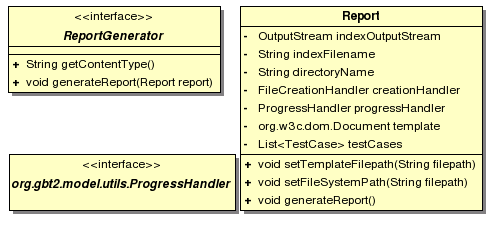
\includegraphics[width=0.9\textwidth]{images/Report/Report.png}
 \caption{\cls{Report}, \itf{ReportGenerator}}
 \label{figure:Classes:Report:Report}
\end{figure}


\paragraph{Fields} \label{Classes:Report:Report:Fields}

Following fields of an \obj{Report} can be set by setter methods and of course they can also be read by getter methods. There is a unusual setter called \mtd{setFileSystemPath(...)} which sets more than one field, it is described in~\ref{Classes:Report:Report:Methods:setFileSystemPath}.

All fields except for \fld{directoryName} must be set in case of multiple-files-report before generating the report by calling \mtd{generateReport()}.

For generation of a single-file-report the fields \fld{directoryName} and \fld{creationHandler} are ignored and thus don't have to be set.

\begin{description}
\item[\fld{indexOutputStream}:] The \obj{OutputStream} where either the index file of a multiple-files-report is written to or the file of the single-file-report is written to.

\item[\fld{indexFilename}:] The name of the index file or the file of the single-file-report as a \obj{String}.

\item[\fld{directoryName}:] The name of the output directory as a \obj{String} where the auxiliary files are written to in case of a multiple-files-report. In case of a single-file-report this field is ignored. If this field is not set it defaults to \mbox{\fld{indexFilename}\texttt{-files}}.

\item[\fld{creationHandler}:] A \pkg{\rootpkg.report.}\imp{FileCreationHandler} (see~\ref{Classes:Report:FileCreationHandler}) which is used to create auxiliary files and thus is only needed for multiple-files-reports and is ignored in case of single-file-reports.

\item[\fld{progressHandler}:] A \pkg{\rootpkg.model.utils.}\imp{ProgressHandler} which is periodically informed about the progress of report generation.

\item[\fld{template}:] The template can either be set as a \obj{String} which points to the template in the filesystem or as a \pkg{org.w3c.dom.}\obj{Document} which allows template generation on the fly without writing it on disk. Internally the template is saved as a \pkg{org.w3c.dom.}\obj{Document}. Thus the setter which receives the \obj{String} has to parse the template file and create a \pkg{org.w3c.dom.}\obj{Document}. This setter is described in~\ref{Classes:Report:Report:Methods:setTemplateFilepath}.

\item[\fld{testCases}:] The content of the report as a \imp{List} of \pkg{\rootpkg.model.}\obj{TestCase}s.
\end{description}


\paragraph{Methods} \label{Classes:Report:Report:Methods}

The setters and getters of the fields listed above are not explicitly defined here but must be implemented of course.


\subparagraph{\mtd{setTemplateFilepath(String filepath)}} \label{Classes:Report:Report:Methods:setTemplateFilepath}

This method creates a \pkg{org.w3c.dom.}\obj{Document} from the template file which can be accessed by the given \code{filepath}. The \pkg{org.w3c.dom.}\obj{Document} is saved into \fld{template}.


\subparagraph{\mtd{setFileSystemPath(String filepath)}} \label{Classes:Report:Report:Methods:setFileSystemPath}

This method is provided for convenience and configures a \obj{Report} to write the report to the given path in the file system. It sets the following fields of a \obj{Report}:
\begin{itemize}
\item \fld{indexFilename}
\item \fld{indexOutputStream}
\item \fld{directoryName} (implicitly set)
\item \fld{creationHandler}
\end{itemize}

The parameter of this method is the path the index file of a multiple-files-report or the file of a single-file-report is written to and is referenced as the \emph{given path} in this section.

This method sets \fld{indexFilename} to the basename of the given path. \fld{indexOutputStream} is set to write to the given path. \fld{directoryName} is not set explicitly here but it defaults to \mbox{\fld{indexFilename}\texttt{-files}} as described in~\ref{Classes:Report:Report:Fields}. The output directory is a directory which name is the value of \fld{directoryName} and which resides in the dirname of the given path. Thus \fld{creationHandler} is set to a \imp{DefaultFileCreationHandler} (see~\ref{Classes:Report:DefaultFileCreationHandler}) with the path to the output directory as the parameter of its constructor.


\subparagraph{\mtd{generateReport()}}

This method hands the report generation over to the \pkg{\rootpkg.report.}\imp{ReportGenerator} the template requires. This works as follows: This method reads the name of the class which will generate the
report from the template. This class must implement \pkg{\rootpkg.report.}\itf{ReportGenerator}. This method instantiates the required \pkg{\rootpkg.report.}\imp{ReportGenerator}, calls \mtd{generateReport(...)} of the \pkg{\rootpkg.report.}\imp{ReportGenerator} and passes the \obj{Report} this method belongs as the parameter. 


\subsubsection{\itf{ReportGenerator}} \label{Classes:Report:ReportGenerator}
\namespace{\pkg{\rootpkg.report.}\itf{ReportGenerator}}

A \imp{ReportGenerator} is responsible for creating a report in a specific format, e.g. hierarchical HTML.

Since the data model of \gbt is designed to be able to save data independently from programming languages this interface can be implemented so that it generates reports for all programming languages supported by \gbt.


\paragraph{\mtd{generateReport(\pkg{\rootpkg.report.}\cls{Report} report)}}
This method generates the report based on the settings saved in the given \obj{Report}. These settings can be retrieved by the getters of the given \obj{Report}.


\paragraph{\mtd{getContentType()}}
This method returns the output format the \imp{ReportGenerator} produces as a MIME content type (e.g. text/plain for plain text).


\subsubsection{\itf{FileCreationHandler}} \label{Classes:Report:FileCreationHandler}

\begin{figure}[hbtp]
 \centering
 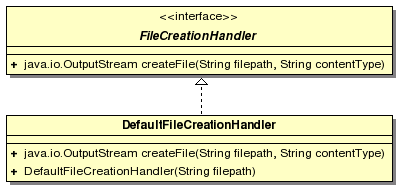
\includegraphics[width=0.8\textwidth]{images/Report/FileCreationHandler.png}
 \caption{\itf{FileCreationHandler}, \cls{DefaultFileCreationHandler}}
 \label{figure:Classes:Report:FileCreationHandler}
\end{figure}

The report component uses the \imp{FileCreationHandler} for creating the auxiliary files of a multiple-files-report. Auxiliary files are saved in the output directory of the report. Thus it is recommended to implement \imp{FileCreationHandler} to create files only in a specific directory, the output directory. A good example is the \cls{DefaultFileCreationHandler} which defines a path in its constructor all created files are saved in.

A \imp{FileCreationHandler} is responsible for creating a file which was requested by calling \imp{FileCreationHandler.}\mtd{createFile(...)}. The parameters of this method are the path to the file and its content-type (e.g. \texttt{text/plain} for plain text). The method returns an \obj{OutputStream} which can be used to write to the newly created file.

% By providing a \imp{FileCreationHandler} to a \imp{ReportGenerator} it is possible to write the generated report to all kinds of data storages because the \imp{ReportGenerator} uses the \imp{FileCreationHandler} to create auxiliary files. Depending on the implementation of \imp{FileCreationHandler.}\mtd{createFile(...)} the report is written to a database, a file, a buffer in memory or whatever the \obj{OutputStream} which is returned by \imp{FileCreationHandler.}\mtd{createFile(...)} points to.


\subsubsection{\cls{DefaultFileCreationHandler}} \label{Classes:Report:DefaultFileCreationHandler}

\cls{DefaultFileCreationHandler} implements \itf{FileCreationHandler} and simply creates files in the file system.

An object is instantiated by using the constructor \cls{DefaultFileCreationHandler.}\mtd{DefaultFileCreationHandler(\cls{String} path)} whereas \code{path} represents the path to the directory files are created in (via \obj{DefaultFileCreationHandler.}\mtd{createFile(...)}). All paths passed to \obj{DefaultFileCreationHandler.}\mtd{createFile(...)} are treated as being relative to the directory set by the constructor. Passing an absolute path to \obj{DefaultFileCreationHandler.}\mtd{createFile(...)} that doesn't point inside the directory set by the constructor is not allowed. This must be considered when implementing \cls{DefaultFileCreationHandler} and can be avoided by throwing an exception for example.


\subsubsection{Template format} \label{Classes:Report:Template}

The format of templates is XML and the general structure is as follows:
\begin{verbatim}
<?xml version="1.0" encoding="UTF-8"?>
<report version="1.0" xmlns="http://www.codecover.org/xml/report-template">
    <class>org.codecover.report.html.HTMLReportGenerator</class>
    <name>HTML Report (hierarchic)</name>
    <description>Generates a hierarchic report in HTML-format.</description>
    <template
      version="1"
      xmlns="http://www.codecover.org/xml/report-template/html-hierarchic">
    ...
    </template>
</report>
\end{verbatim}
All of the above defined elements and attributes are required in a template (non is optional). It is recommended but not required to use UTF-8 as the character encoding.

The element \code{class} defines the fully qualified name of the class which can process the template. This class must implement \pkg{\rootpkg.report.}\itf{ReportGenerator}. In the above example it is the class \pkg{org.codecover.report.html.}\cls{HTMLReportGenerator}.

The attribute \code{version} of the root element \code{report} sets the version of the template format. The template format which is specified in this document has the version 1.0. The version is read by \pkg{\rootpkg.report.}\cls{Report.}\mtdst{generateReport(...)} and compared to the internal version number of the report component. The major version number is incremented if a change in the component happens that requires restructuring the template format so that it is incompatible with the component before the change. If only minimal changes to the template format happen which don't affect the compatibility then the minor version number is incremented. This is the case if for example new elements are added to the template. An older version of the report component can't process these new elements  but it still must be able to process the template and create a report. Changes to the structure inside the \code{template} element don't affect the version number because this structure is specific to the class which generates the report.

The namespace of the root element is defined in its attribute \code{xmlns} and must be \texttt{http://www.codecover.org/xml/report-template}.

The name of the template is set with the element \code{name} and a short description is set with the element \code{description}. The language for both must be english.

The attribute \code{version} of the element \code{template} sets the version of the template and is specific to the class which generates the report. It is recommended to use this version in the implementation of a report generating class to assure compatibility of the template and the class.

The content of the element \code{template} (indicated by \code{...} in the above example) is specific to the class which generates the report. Typically the element \code{template} contains a new level of subelements and these subelements contain CDATA-sections which contain the real templates with placeholders, see~\ref{Classes:Report:HTMLReport} for an example. The namespace of the element \code{template} is defined in its attribute \code{xmlns}. It must be unique and is recommended to be \texttt{http://www.codecover.org/xml/report-template/} plus a name of the output format of the template. For example the hierarchic HTML Report uses \texttt{html-hierarchic} as the name and the full namespace is \texttt{http://www.codecover.org/xml/report-template/html-hierarchic}.

If the template is saved as a file in the filesystem the recommended filename is the name defined in element \code{name} whereas spaces are translated to underscores and potentially problematic characters like /, $\backslash$ and other non-basic latin letters should be avoided in the filename. The recommended file extension is \texttt{codecovertmpl}. The filename for the hierarchic HTML Report is \texttt{HTML\_Report\_hierarchic.codecovertmpl} for example.


\subsubsection{Extensibility}
\namespace{\pkg{\rootpkg.report}}

To extend the report component you have to write a new class which implements \itf{ReportGenerator} (\ref{Classes:Report:ReportGenerator}). It is recommended but not required to put this new class into a package which is named after the output format of the new class, e.g. \pkg{html} (see~\ref{Classes:Report:HTMLReport}), and to put this new package into \pkg{\rootpkg.report}. Moreover a new template format has to be specified considering the specification in~\ref{Classes:Report:Template}.


\subsubsection{Hierarchic HTML Report} \label{Classes:Report:HTMLReport}
\namespace{\pkg{\rootpkg.report.html}}

The hierarchic HTML report is realized by \cls{HTMLReportGenerator} which implements \pkg{\rootpkg.report.}\itf{ReportGenerator}. Apache Velocity\footnote{Apache Velocity: http://velocity.apache.org/} is used as the template engine.

The template format is extended as follows:
\begin{verbatim}
<?xml version="1.0" encoding="UTF-8"?>
<report version="1.0" xmlns="http://www.codecover.org/xml/report-template">
    <class>org.codecover.report.html.HTMLReportGenerator</class>
    <name>HTML Report (hierarchic)</name>
    <description>Generates a hierarchic report in HTML-format.</description>
    <template
      version="1"
      xmlns="http://www.codecover.org/xml/report-template/html-hierarchic">
        <title-page><![CDATA[
            ...
        ]]></title-page>
        <selection-page><![CDATA[
            ...
        ]]></selection-page>
        <code-page><![CDATA[
            ...
        ]]></code-page>
    </template>
</report>
\end{verbatim}
The filename of the template is \texttt{HTML\_Report\_hierarchic.codecovertmpl}.

The version number defined in the attribute \code{version} of element \code{template} must be incremented if any changes to the HTML report generation happen that affect the structure or semantics of placeholders inside the element \code{template}.

There are three new elements which contain the template HTML code for title (\code{title-page}), selection (\code{selection-page}) and code pages (\code{code-page}). The HTML code of the template contains placeholders for the data which will be inserted in the template by Apache Velocity. This works as follows:
\begin{enumerate}
\item An instance of the Apache Velocity template engine is created.
\item A so-called Context is filled with the data that will be inserted into the template HTML code for the title page. This is done by saving the actual value and a key to this value. The key of the value is the name of the placeholder in the template HTML code.
\item The template HTML code is \emph{merged} with the Context, that is the placeholders are replaced with the real data.
\item Now a Context is created for each selection page. In case of Java it is a Context for each package. In case of COBOL this and the next step are skipped because there are no selection pages for COBOL.
\item The Contexts are merged with the template HTML code for selection pages. This creates the selection pages of the report.
\item Now a Context is created for each code page. In case of Java it is a Context for each class. In case of COBOL it is a Context for each section.
\item The Contexts are merged with the template HTML code for code pages. This creates the code pages of the report.
\end{enumerate}

\fussy


\subsection{Batch}
\namespace{\pkg{\rootpkg.batch}}

\begin{figure}[hbtp]
 \centering
 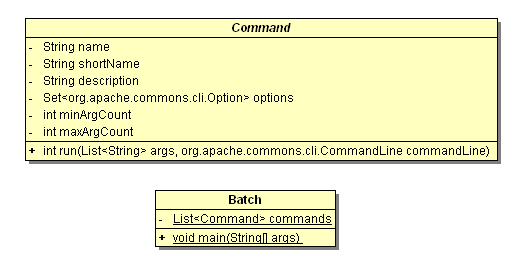
\includegraphics[width=0.7\textwidth]{images/Batch/batch.png}
 \caption{\pkg{\rootpkg.batch}}
 \label{figure:Classes:Batch}
\end{figure}

The batch interface uses
\linkwithfootnote{http://jakarta.apache.org/commons/cli/}{Jakarta Commons CLI}
with the
\linkwithfootnote{http://jakarta.apache.org/commons/cli/apidocs/org/apache/commons/cli/PosixParser.html}{POSIX parser}
to parse the command line options.

\subsubsection{\clsab{Command}}

A \obj{Command} represents a \gbt batch command (like e.g. \code{instrument}
or \code{info}).

It has a name (e.g. \code{instrument}), eventually a short name (e.g.
\code{in}), a description (e.g. \code{instrumentation of code files}), a
set of references to the accepted options (which are references to \obj{Option}
objects of the Jakarta Commons CLI library) and a minumum and maximum number of
parameters accepted by the command. The maximum number can be \code{-1}
to indicate that there is no upper limit.

\mtdab{run(...)} will be called when the command is executed.

The various commands will be implemented by anonymous classes extending this
class.

\subsubsection{\cls{Batch}}

This is the main batch class.

It contains a list of \obj{Command}s and the \mtdst{main(...)} method.

\subsection{Eclipse} \label{Eclipse}
The design of the Eclipse plugin part of \gbt is rather coarse, the design team decided that it is unnecessary to model e.g. the GUI part in greater detail, also because the GUI has been specified very detailed in the specification. For the same reason the classes are only listed in their corresponding packages, without providing any class diagram.

\def\extpoint#1{
\item \code{org.eclipse.#1}
}

\par The listed Eclipse Extension Points for each package are subject to change, a final decision will be made during the implementation.

\namespace{\pkg{\rootpkg.eclipse}}
This package contains all the packages and classes which are related to the Eclipse plugin part of \gbt.
\cls{InstrumentableItem} represents an item which can be selected for instrumentation, e.g. a source file or a package. \cls{CoverageMode} is similar to the standard Eclipse Run mode, except that the source files are instrumented and coverage data is collected during runtime.

Probably the following Eclipse Extension Points will be used for this package:
\begin{itemize}
\extpoint{core.runtime.adapters}
\extpoint{debug.ui.launchGroups}
\extpoint{debug.ui.launchShortcuts}
\extpoint{debug.ui.launchConfigurationTabGroups}
\extpoint{debug.core.statusHandlers}
\end{itemize}


\namespace{\pkg{\rootpkg.eclipse.actions}}
This package will contain classes which implement the behaviour of e.g. menu items or toolbar items.

Probably the following Eclipse Extension Points will be used for this package:
\begin{itemize}
\extpoint{ui.actionSets}
\extpoint{ui.commands}
\end{itemize}

\namespace{\pkg{\rootpkg.eclipse.dialogs}}
This package contains classes for all the required dialogs:
\begin{itemize}
\item \cls{InstrumentationDialog}
\item \cls{ImportSessionDialog}
\item \cls{ImportCoverageResultsDialog}
\item \cls{ReportDialog}
\item \cls{ExportSessionDialog}
\item \cls{TestCasePropertiesDialog}
\item \cls{PreferencesDialog}
\item \cls{ProjectPropertiesDialog}
\end{itemize}
Probably the following Eclipse Extension Points will be used for this package:
\begin{itemize}
\extpoint{core.runtime.preferences}
\extpoint{ui.importWizards}
\extpoint{ui.exportWizards}
\end{itemize}

Detailed information about a certain dialog can be found in the specification.
\namespace{\pkg{\rootpkg.eclipse.controls}}
This package will contain custom controls, e.g. a control for the correlation matrix planned for a later iteration.
\namespace{\pkg{\rootpkg.eclipse.views}}
This package contains \cls{SessionView} and \cls{CoverageView}. Detailed information about these views can be found in the specification.

\par Probably the following Eclipse Extension Points will be used for this package:
\begin{itemize}
\extpoint{ui.views}
\extpoint{ui.editors.markerAnnotationSpecification}
\extpoint{ui.editors.documentProviders}
\extpoint{ui.perspectives}
\extpoint{ui.perspectiveExtensions}
\end{itemize}

%\svnid{$Id: Activities.tex 1 2007-12-12 17:37:26Z t-scheller $}
\section{Activity diagrams} \label{Activities}

This section contains the activity diagrams created from the specification. They represent a more formal depiction of the use cases listed in the specification and they contain the pre- and postconditions, the regular sequence, as well as the possible exceptions described there.

\clearpage
\subsection{Analyze coverage log}
\begin{figure}[htb]
 \centering
 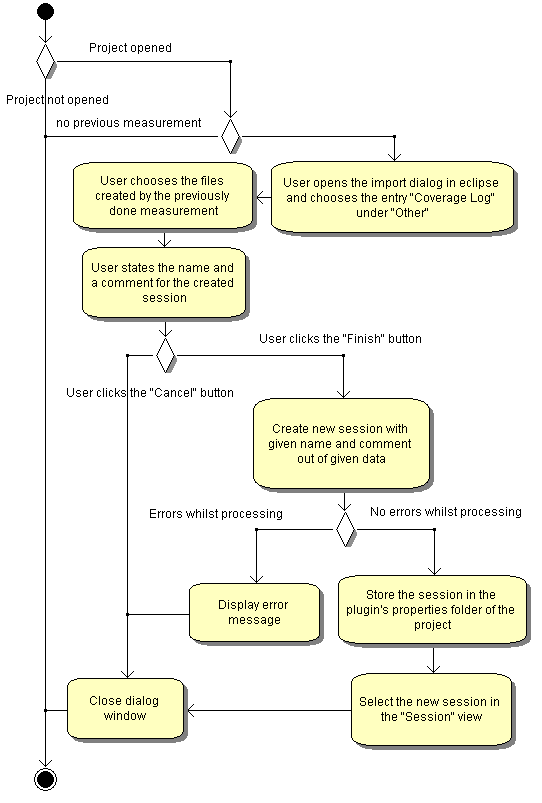
\includegraphics[height=0.7\textheight]{images/Activities/analyze_coverage_log.png}
 \caption{Analyze coverage log}
 \label{ac_fg:analyze}
\end{figure}

\clearpage
\subsection{Associate test case}
\begin{figure}[htb]
 \centering
 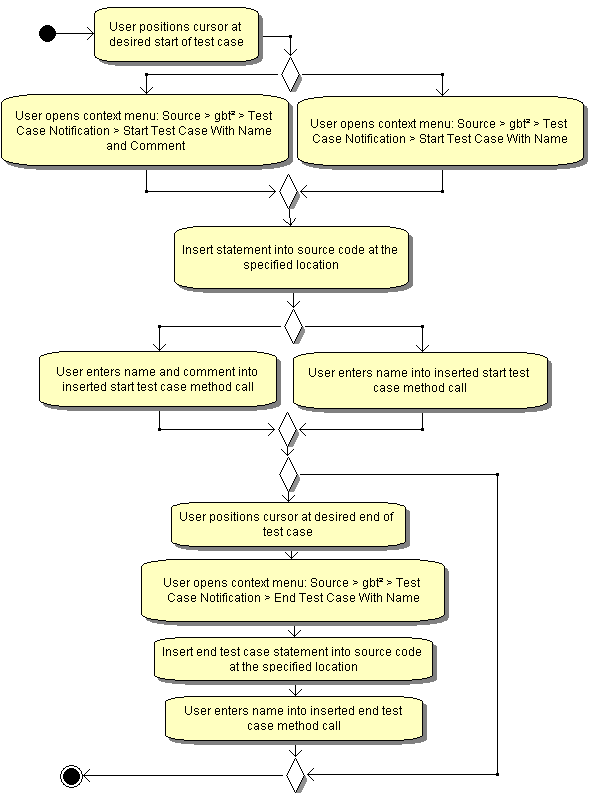
\includegraphics[height=0.7\textheight]{images/Activities/associate_test_case.png}
 \caption{Associate test case}
 \label{ac_fg:associate}
\end{figure}

\clearpage
\subsection{Configure preferences}
\begin{figure}[htb]
 \centering
 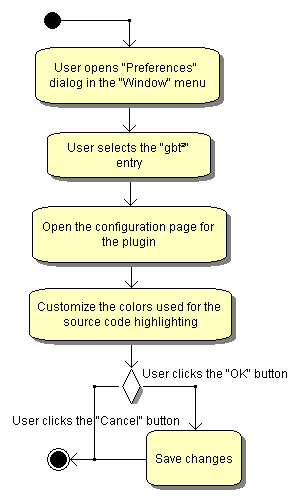
\includegraphics[height=0.7\textheight]{images/Activities/configure_preferences.png}
 \caption{Configure preferences}
 \label{ac_fg:preferences}
\end{figure}

\clearpage
\subsection{Drop session}
\begin{figure}[htb]
 \centering
 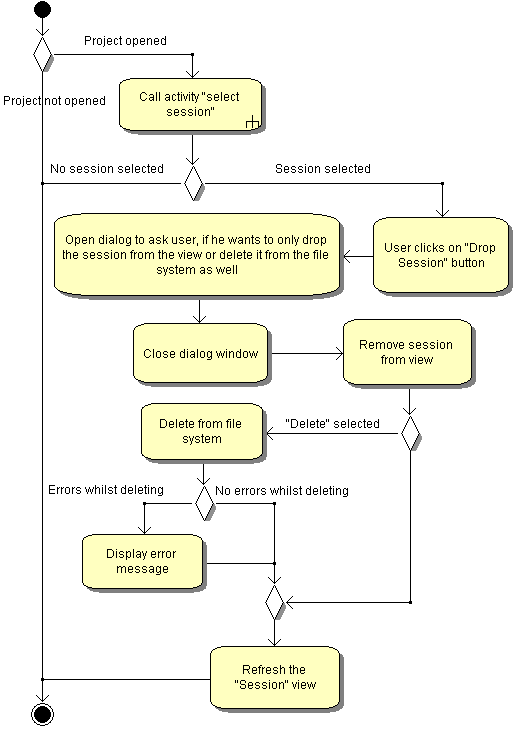
\includegraphics[height=0.7\textheight]{images/Activities/drop_session.png}
 \caption{Drop session}
 \label{ac_fg:drop_session}
\end{figure}

\clearpage
\subsection{Drop test case}
\begin{figure}[htb]
 \centering
 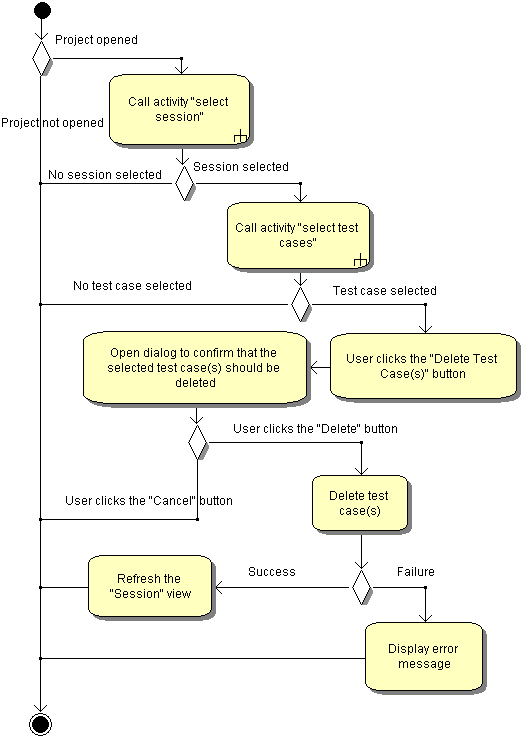
\includegraphics[height=0.7\textheight]{images/Activities/drop_test_case.png}
 \caption{Drop test case}
 \label{ac_fg:drop_test_case}
\end{figure}

\clearpage
\subsection{Edit session properties}
\begin{figure}[htb]
 \centering
 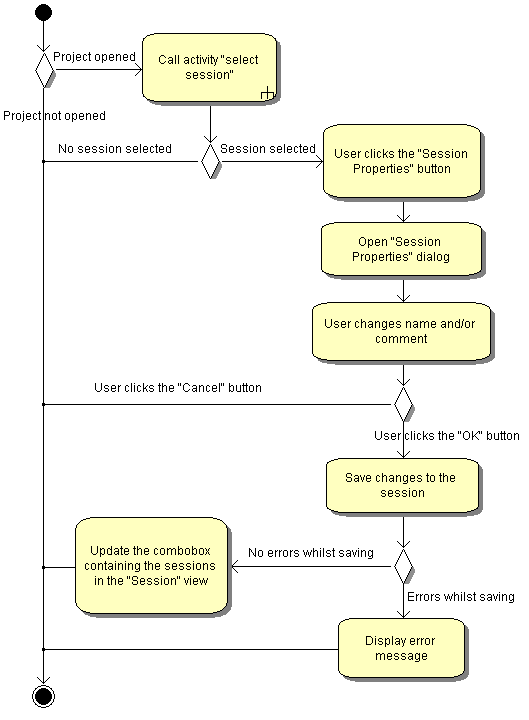
\includegraphics[height=0.7\textheight]{images/Activities/edit_session_properites.png}
 \caption{Edit session properties}
 \label{ac_fg:edit_session}
\end{figure}

\clearpage
\subsection{Edit test case properties}
\begin{figure}[htb]
 \centering
 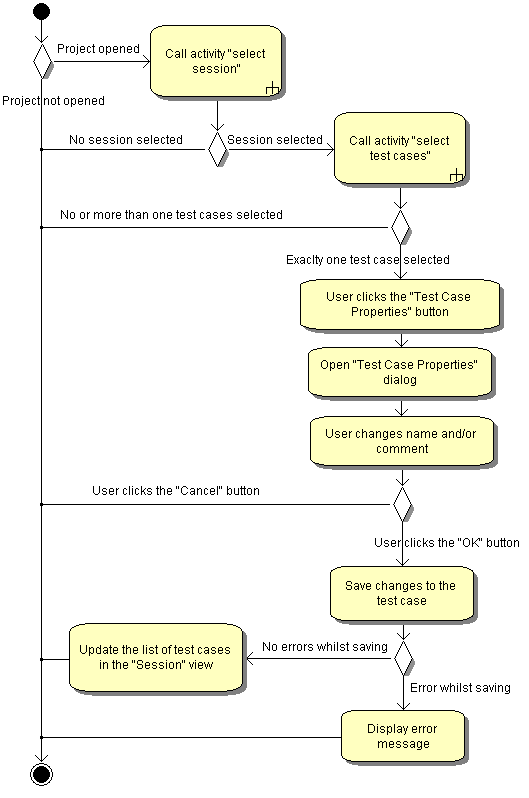
\includegraphics[height=0.7\textheight]{images/Activities/edit_test_case_properties.png}
 \caption{Edit test case properties}
 \label{ac_fg:edit_test_case}
\end{figure}

\clearpage
\subsection{Export session}
\begin{figure}[htb]
 \centering
 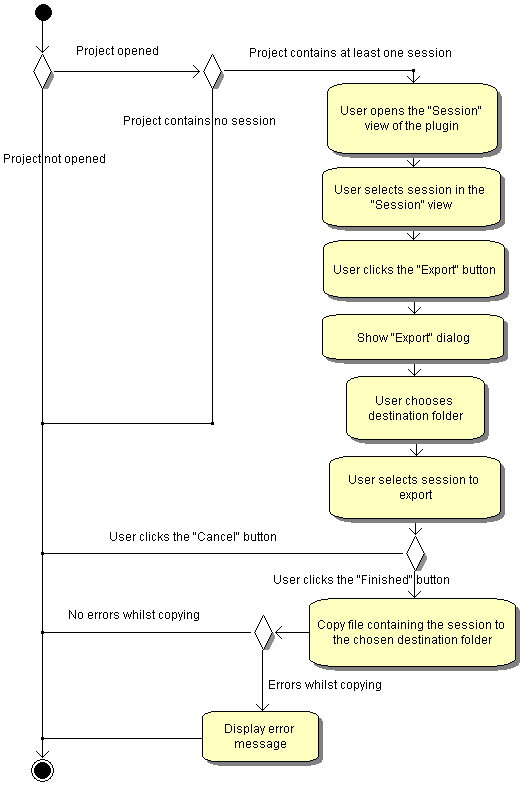
\includegraphics[height=0.7\textheight]{images/Activities/export_session.png}
 \caption{Export session}
 \label{ac_fg:export}
\end{figure}

\clearpage
\subsection{Generate report}
\begin{figure}[htb]
 \centering
 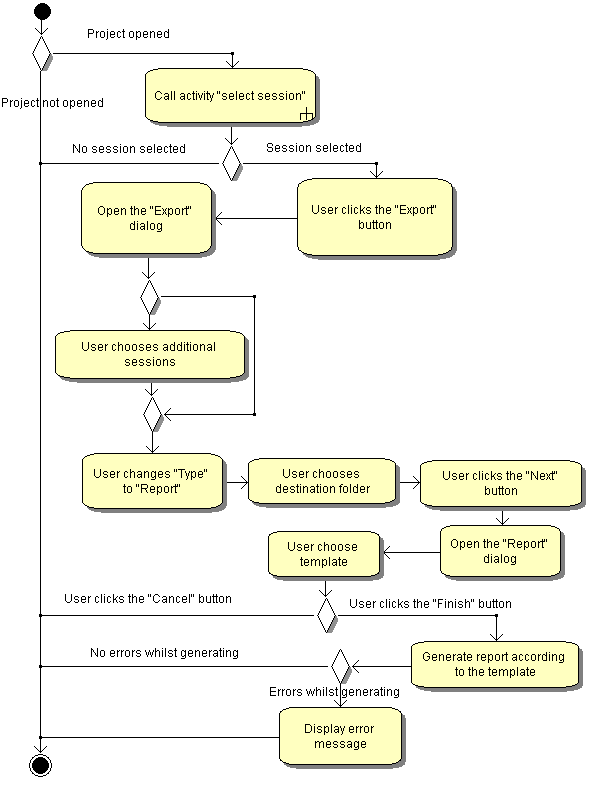
\includegraphics[height=0.7\textheight]{images/Activities/generate_report.png}
 \caption{Generate report}
 \label{ac_fg:report}
\end{figure}

\clearpage
\subsection{Import session}
\begin{figure}[htb]
 \centering
 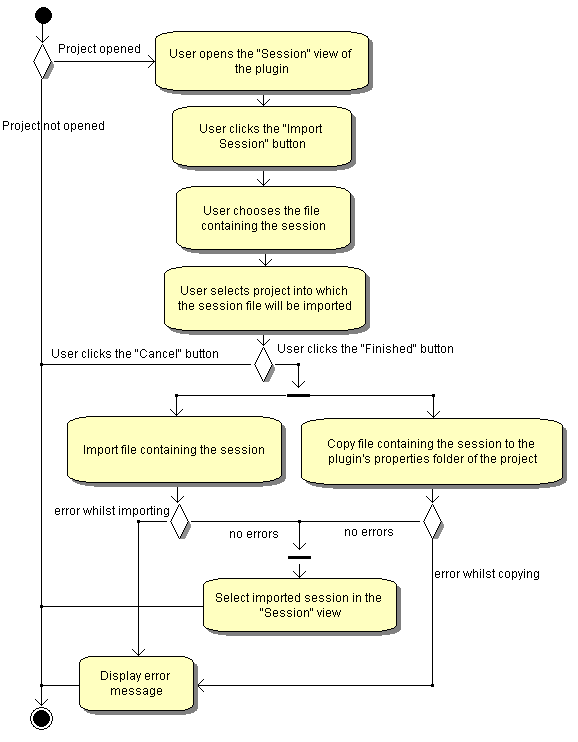
\includegraphics[height=0.7\textheight]{images/Activities/import_session.png}
 \caption{Import session}
 \label{ac_fg:import}
\end{figure}

\clearpage
\subsection{Instrument instrumentable items}
\begin{figure}[htb]
 \centering
 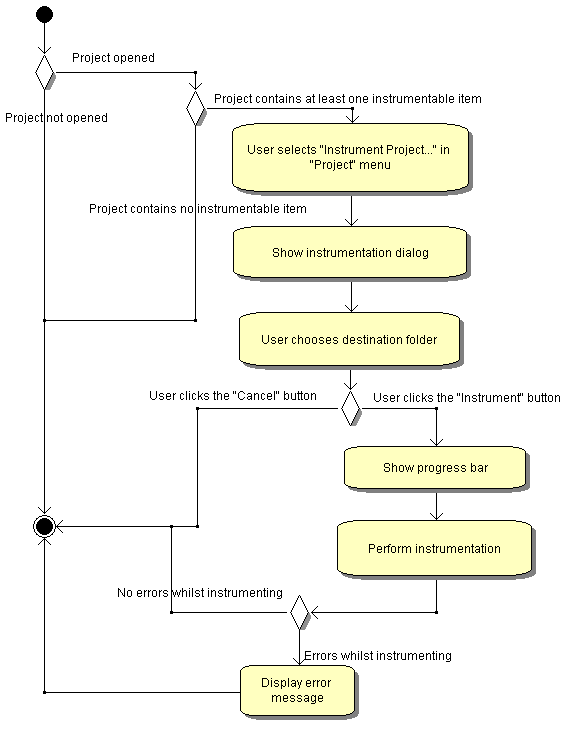
\includegraphics[height=0.7\textheight]{images/Activities/insturment_instrumentable_items.png}
 \caption{Instrument instrumentable items}
 \label{ac_fg:instrument_items}
\end{figure}

\clearpage
\subsection{Measure coverage}
\begin{figure}[htb]
 \centering
 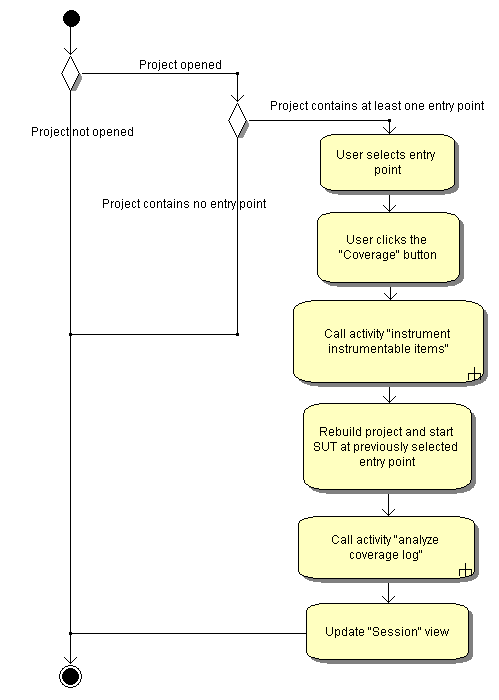
\includegraphics[height=0.7\textheight]{images/Activities/measure_coverage.png}
 \caption{Measure coverage}
 \label{ac_fg:measure}
\end{figure}

\clearpage
\subsection{Merge sessions}
\begin{figure}[htb]
 \centering
 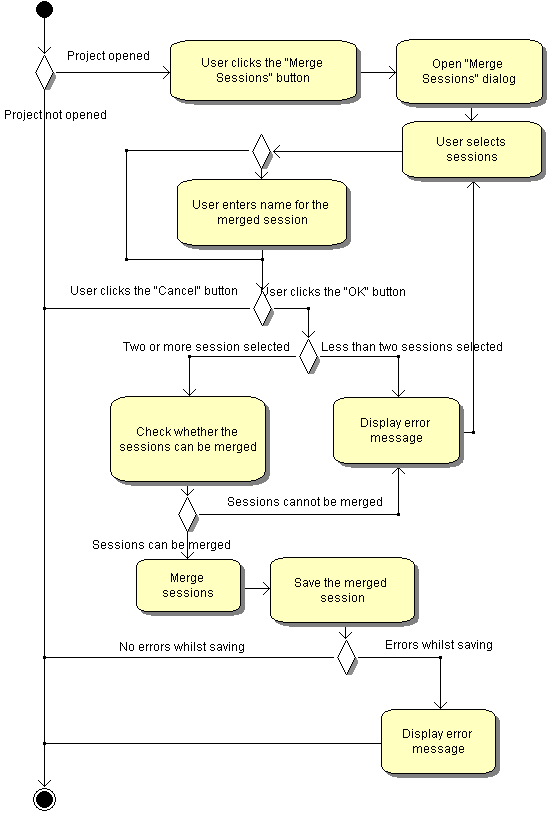
\includegraphics[height=0.7\textheight]{images/Activities/merge_sessions.png}
 \caption{Merge sessions}
 \label{ac_fg:merge_sessions}
\end{figure}

\clearpage
\subsection{Merge test cases}
\begin{figure}[htb]
 \centering
 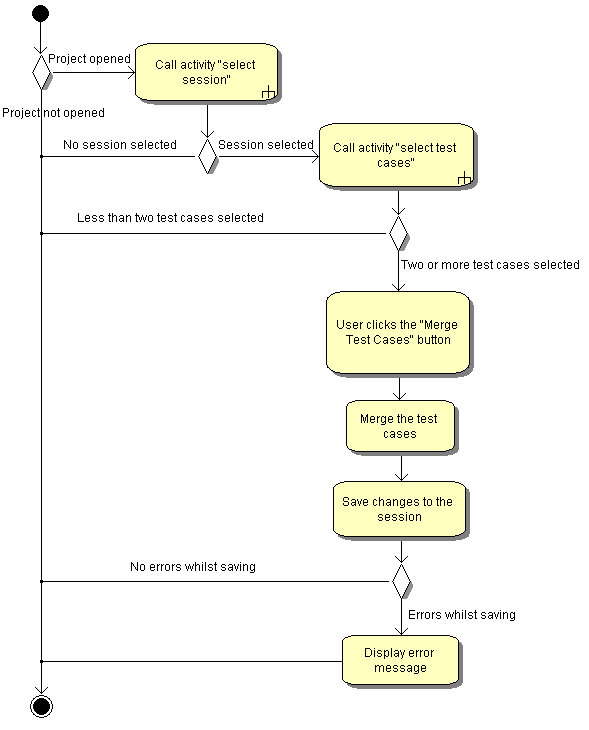
\includegraphics[height=0.7\textheight]{images/Activities/merge_test_cases.png}
 \caption{Merge test cases}
 \label{ac_fg:merge_test_cases}
\end{figure}

\clearpage
\subsection{Select coverage criteria}
\begin{figure}[htb]
 \centering
 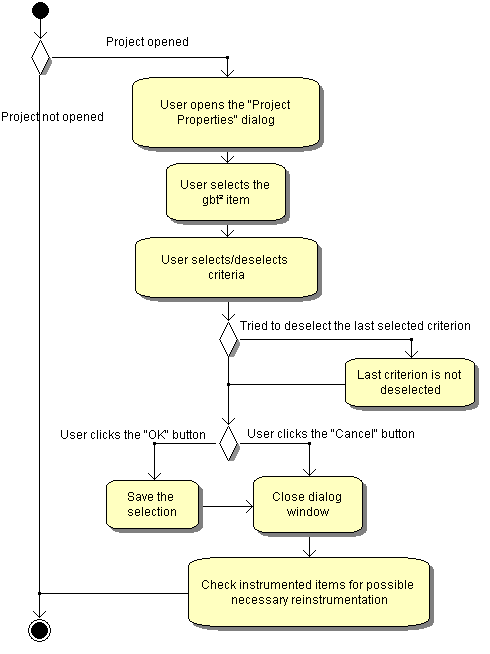
\includegraphics[height=0.7\textheight]{images/Activities/select_coverage_criteria.png}
 \caption{Select coverage criteria}
 \label{ac_fg:select_coverage}
\end{figure}

\clearpage
\subsection{Select instrumentable items}
\begin{figure}[htb]
 \centering
 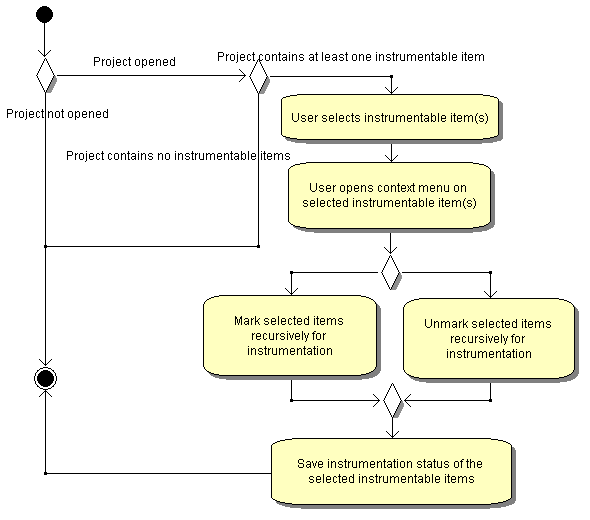
\includegraphics[height=0.7\textheight]{images/Activities/select_instrumentable_items.png}
 \caption{Select instrumentable items}
 \label{ac_fg:select_items}
\end{figure}

\clearpage
\subsection{Select session}
\begin{figure}[htb]
 \centering
 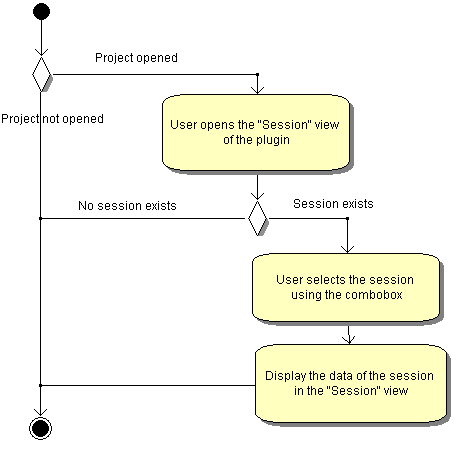
\includegraphics[height=0.7\textheight]{images/Activities/select_session.png}
 \caption{Select session}
 \label{ac_fg:select_session}
\end{figure}

\clearpage
\subsection{Select test cases}
\begin{figure}[htb]
 \centering
 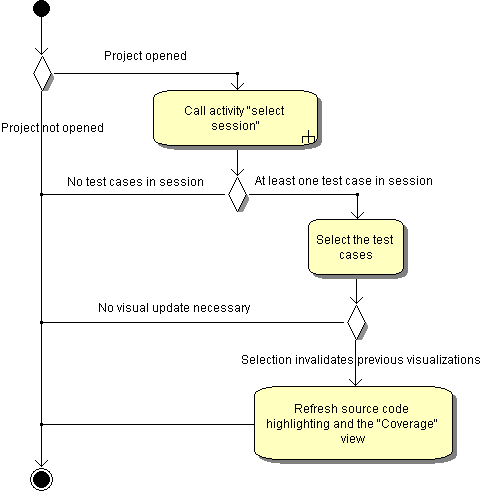
\includegraphics[height=0.7\textheight]{images/Activities/select_test_cases.png}
 \caption{Select test cases}
 \label{ac_fg:select_test_cases}
\end{figure}

\clearpage
\subsection{Show coverage measurement}
\begin{figure}[htb]
 \centering
 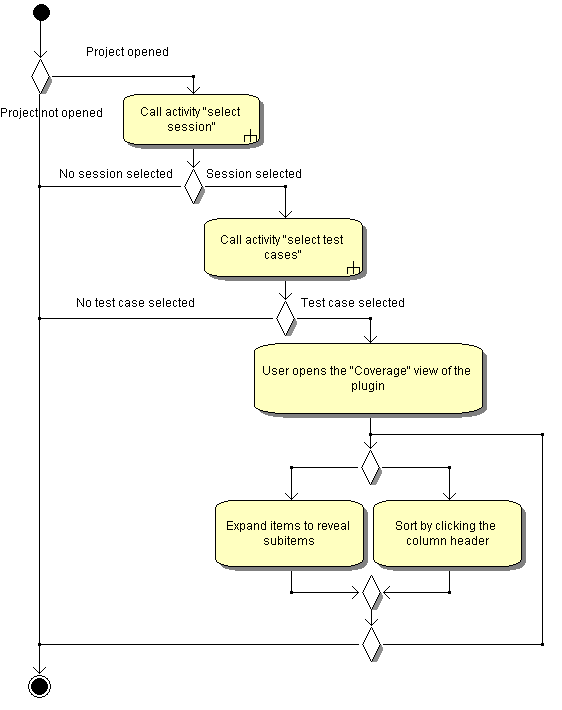
\includegraphics[height=0.7\textheight]{images/Activities/show_coverage_measurement.png}
 \caption{Show coverage measurement}
 \label{ac_fg:show coverage}
\end{figure}

\clearpage
\subsection{Show covered code}
\begin{figure}[htb]
 \centering
 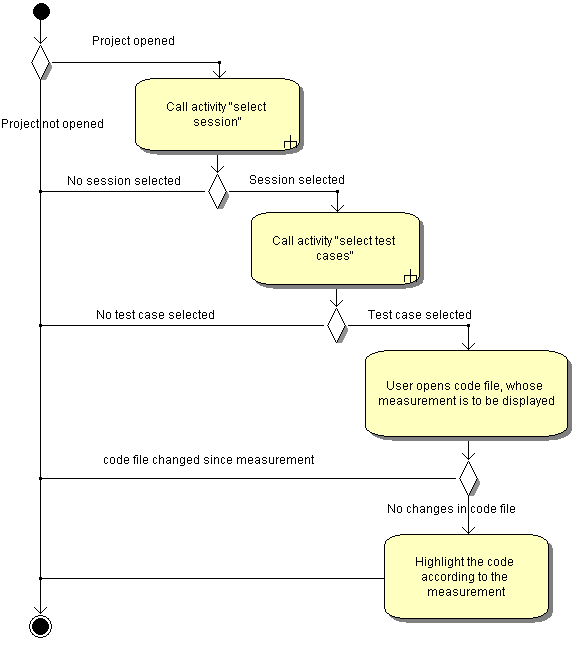
\includegraphics[height=0.7\textheight]{images/Activities/show_covered_code.png}
 \caption{Show covered code}
 \label{ac_fg:show_covered_code}
\end{figure}


% --- List of figures --- %

\newpage
% \phantomsection is needed for correct PDF link to the LOF
% (see specification Bug 2)
\phantomsection
\listoffigures
%\addcontentsline{toc}{section}{List of figures}

\end{document}

%%% Local Variables:
%%% TeX-PDF-mode: t
%%% End:
